\documentclass[slug=GL, room=HZDR\ Dresden/Rossendorf\,\ Geb.\ 540/239, supervisor=Tim\ Ziegler, coursedate=25.\ 10.\ 2019]{../../Lab_Report_LaTeX/lab_report}

\title{Gaslaser}
\author{Oliver Matthes, Valentin Boettcher}
\usepackage[version=4]{mhchem}
\usepackage{todonotes}
\usepackage{amssymb}
\usepackage{graphicx,wrapfig}
\graphicspath{ {figs/} }
\newcommand{\laser}{\textsc{Laser}}
\newcommand{\hne}{\ce{HeNe}-Laser}
\usepackage[ngerman]{babel}

% bib
\addbibresource{protokoll.bib}

\newtheorem{acro}{Acronym}[section]
\begin{document}
\maketitle

\section{Einleitung}%
\label{sec:intro}
Der \laser{} ist seit seiner Erfindung in den 1960er Jahren in der
modernen Physik zu einem Standardwerkzeug geworden. Unter anderem
kann ein Laserstrahl zur Erzeugung von sehr tiefen Temperaturen
(Untersuchung von Quanteneffekten, Bose-Einstein Kondensation), zur
Erzeugung und Untersuchung von Schockwellen und zur Beschleunigung von
Elementarteilchen genutzt werden.

Auch in der Technik findet der \laser{} aufgrund der hohen Koh\"arenz
und Intensität des emittierten Lichtstrahls vielfach Anwendung. So
hat man allt\"aglich mit auf Lasertechnologie basierenden
Barcode-Scannern und CD-Spielern zu tun. Auch die moderne
Telekommunikationstechnik um das Internet nutzt \laser{} zur
Daten\"ubertragung.

Zum n\"aheren Verst\"andnis sollte zun\"achst das Akronym \laser{}
gekl\"art werden.

\begin{acro}[Laser]
\textsc{Light Amplification by Stimulated Emission of Radiation.}
\end{acro}

Dementsprechend verst\"arkt ein \laser{} also Licht durch stimulierte
Emission. Da die stimulierte Emission von Strahlung ein Photon in
allen seinen Eigenschaften kopiert, wird im Allgemeinen koh\"arentes
und bedingt durch die Verst\"arkung sehr intensives Licht erzeugt.

Der grundlegende Aufbau eines Lasers ist erstaunlich einfach. So
besteht ein Laser aus:

\begin{enumerate}
\item einem aktiven Medium (Gase, Festkörper)
\item einem optischen Resonator (meist rotationssymmetrische, sph\"arische Spiegel)
\item einer ``Energiepumpe'' (Lichtblitze, Elektronenst\"oße)
\end{enumerate}

\begin{figure}[H]\centering
  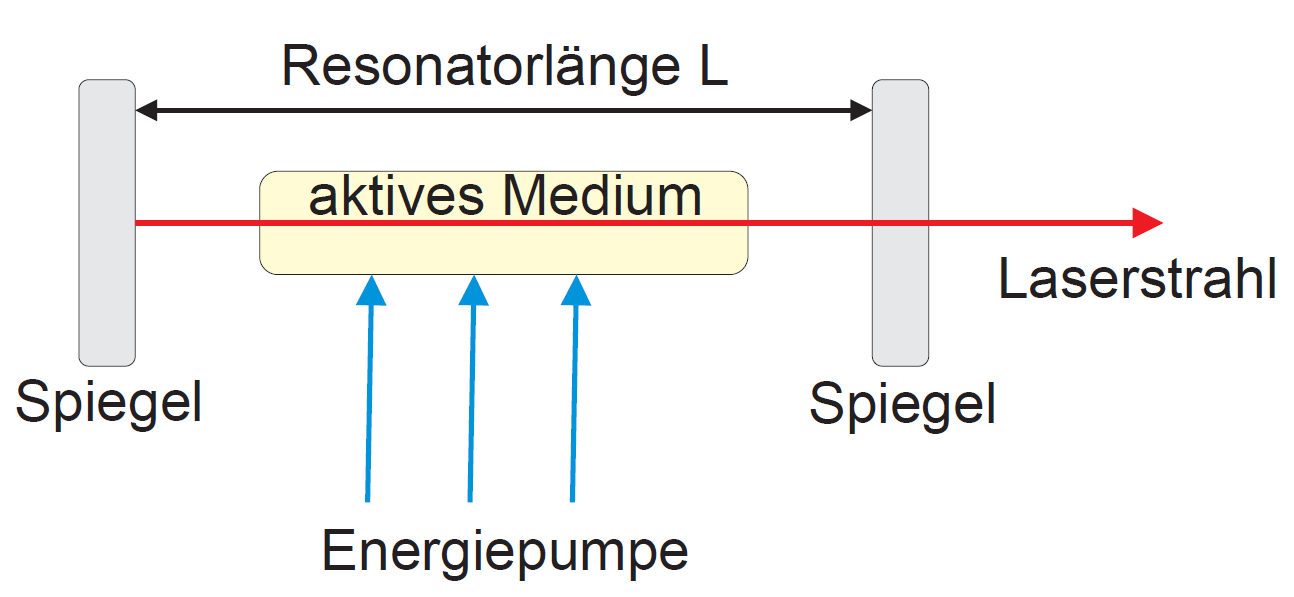
\includegraphics[width=.5\columnwidth]{schema.png}
  \caption[Aufbau]{Schema eines Lasers}
  \label{fig:aufb}
\end{figure}

Die Energiepumpe erzeugt im aktiven Medium eine
Ungleichgewichtsbesetzung von Energieniveaus, die die induzierte
Emission beg\"unstigt. Die Photonen oszillieren im Resonator mehrfach
und werden bei jedem Durchlauf verst\"arkt, bis sie den
Resonator verlassen.

\section{Theoretische Grundlagen}%
\label{sec:theo}

\subsection{Besetzungsinversion und Laserbedingung}%
\label{sec:inv}

Die Elektronen in Atomen nehmen nach der Quantenmechanik nur diskrete
Energien an. Wenn ein Elektron seinen Zustand wechselt, wird bei
diesem \"Ubergang Licht emmitiert oder absorbiert wobei f\"ur die
Energien \(E_i\) und die Frequenz des beteiligten Photons \(\nu\) gilt:

\begin{equation}
  \label{eq:transfreq}
  h\nu = E_2 - E_1
\end{equation}

Es gibt drei Prozesse, die nun die Anzahl der Atome im Grundzustand
\(N_1\) und der angeregten Atome \(N_2\) beeinflussen.

\begin{description}
\item[Absorbtion] Ein Photon wird von einem Atom absorbiert, welches
  dementsprechend angeregt wird. Die H\"aufigkeit dieses Prozesses ist
  proportional zur spektralen Energiedichte.
\item[Spontane Emission] Ein angeregtes Atom geht in einen tieferen
  Zustand \"uber und sendet ein Photon aus. Dieser Prozess ist
  unabh\"angig von der umgebenden spektralen Energiedichte.
\item[Stimulierte Emission] Das Atom wird von einem passenden Photon
  zur Emmission eines zweiten, identischen Photons angeregt und geht
  in einen tieferen Zustand \"uber. Die H\"aufigkeit dieses Prozesses ist
  proportional zur spektralen Energiedichte.
\end{description}

Durch Aufstellung von Ratengleichungen f\"ur das thermische
Gleichgewicht in einem Zweiniveausystem wird deutlich, dass in einem
solchen Fall die spontane Emmission \"uberwiegt und keine
Verst\"arkung auftreten kann, da die Wahrscheinlichkeit f\"ur Absorbtion
und stimulierte Emmision gleich, sowie immer mehr Teilchen im
Grundzustand als im angeregten Zustand sind.

F\"ur die Photonenzahldichte \(q\) gilt mit der spektralen
Energiedichte \(\rho(\nu)\) und dem Einsteinkoeffizienten f\"ur
stimulierte Emission und unter Vernachl\"assigung der spontanen
Emission:

\begin{equation}
  \label{eq:qrate}
  \dv{q}{t}=\rho(\nu)B_{21}(N_2-N_1)
\end{equation}

Damit eine Verst\"arkung auftritt muss gelten:

\begin{equation}
  \label{eq:first}
  \tag{Erste Laserbedingung}
  N_2>N_1
\end{equation}

Eine Besetzungsinversion kann erst mit einem Dreiniveausystem
hergestellt werden. Da dort allerdings das untere Laserniveau der
Grundzustand ist, w\"are eine sehr hohe Pumprate notwendig. Bei einem
Vierniveausystem kann man durch die Nutzung eines selten thermisch
besetzten Niveaus schon mit relativ geringen Pumpraten eine
Besetzungsinversion erzeugen.

\begin{figure}[H]\centering
  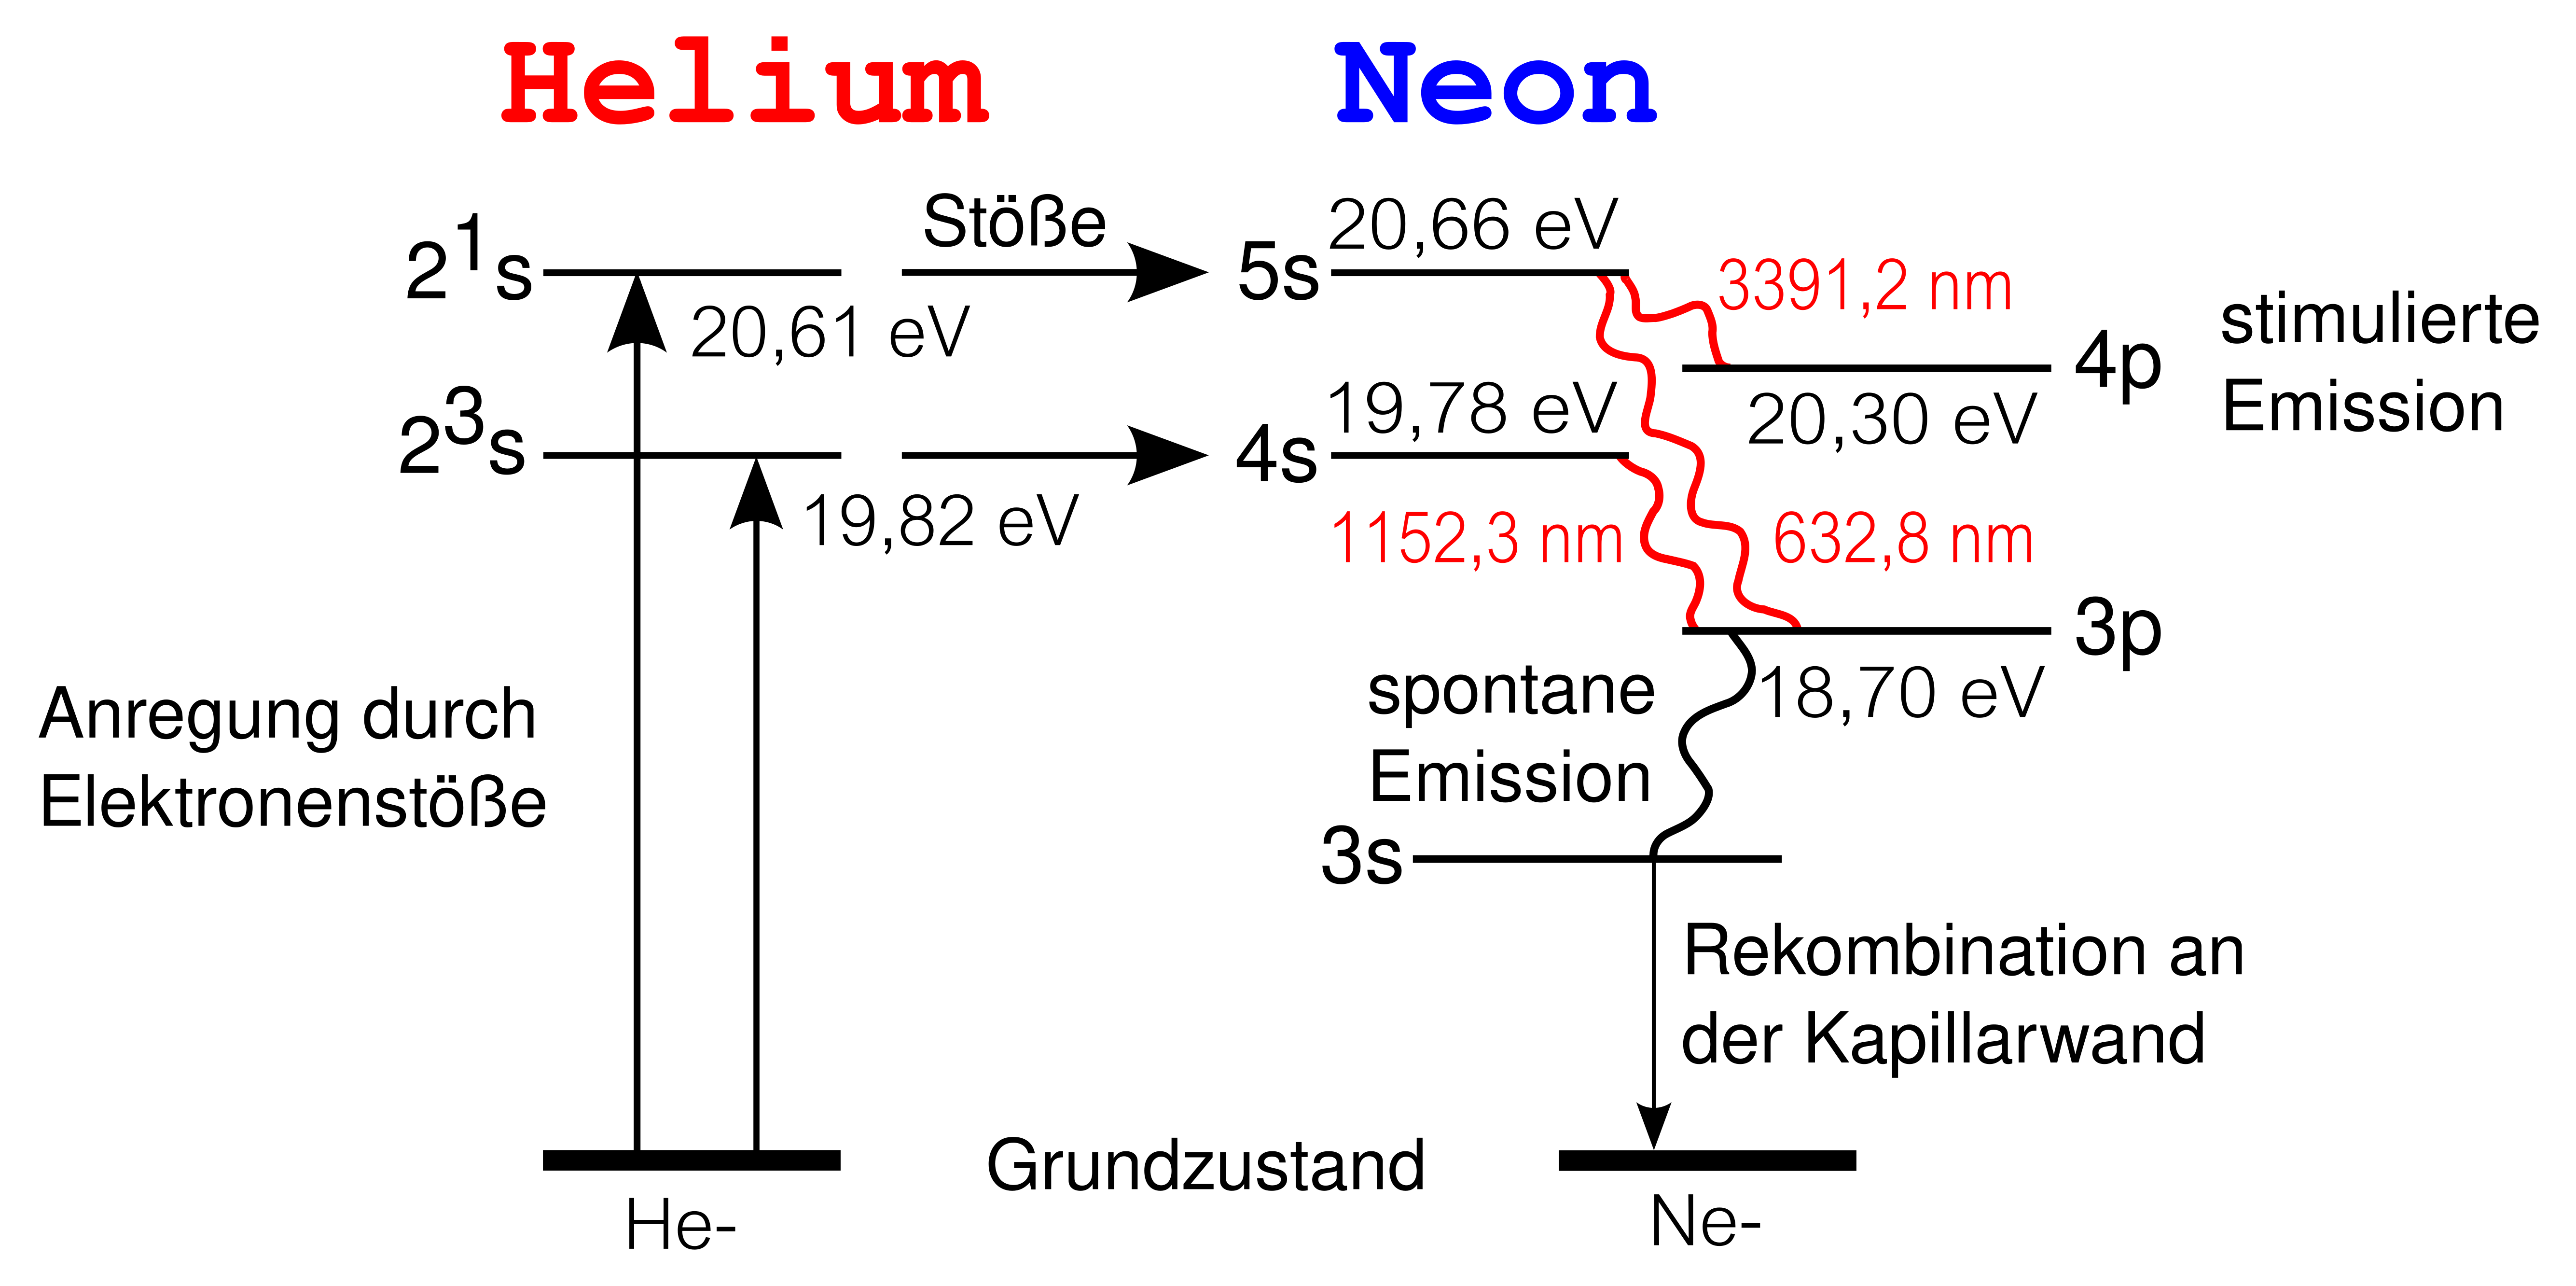
\includegraphics[width=.8\columnwidth]{heneniv.png}
  \caption[Aufbau]{Vierniveausystem des \hne{}}
  \label{fig:niveaus}
\end{figure}

Der \hne{} basiert auf dem in~\ref{fig:niveaus} dargestellten
Vierniveausystem. Das Helium wird (z.B. mit Elektronenst\"o\ss{}en)
angeregt (nach \(2^1S\) bzw. \(2^3S\)) und \"ubertr\"agt diese
Anregungung durch Atomst\"o\ss{}e an das Neon, dessen Niveaus (\(5S\),
\(4S\)) \"ahnlich liegen. Der im optisch sichtbaren Bereich liegende
\"Ubergang \(5S\rightarrow 3P\) wird vorwiegend im \hne{} genutzt und
ist f\"ur eine Besetzungsinversion besonders vorteilhaft, da die
Lebensdauer der \(S\) Niveaus h\"oher als die der \(P\) Niveaus ist.


Um nun die Verst\"arkungswirkung des Lasers in Anwendungen zu nutzen,
ist eine Betrachtung von Energieverlusten n\"otig. \"Ublicherweise
durchqueren Photonen einen Resonator der L\"ange \(L\) mehrfach und
werden dabei durch stimulierte Emission verst\"arkt. Allerdings treten
auch immer Verluste auf, sodass pro doppelten Umlauf die
Intensit\"at um einen Faktor \(e^{-\kappa}\) korrigiert werden muss,
wobei \(\kappa\) der sog. Verlustkoeffizient ist. Nach dieser
Betrachtung muss die Verst\"arkung gr\"o\ss{}er sein als der Verlust.
Mit dem Wirkungsquerschnitt \(\sigma_{21}=B_{21}\frac{h\cdot\nu}{c}\)
ergibt sich:

\begin{equation}
  \label{eq:zwlabe}
  \tag{zweite Laserbedingung}
  \sigma_{21}(N_2-N_1)\cdot 2L \geq \kappa
\end{equation}

Falls nur Verluste bei der Reflexion an den Resonatorspiegeln
auftreten, gilt mit den Reflexionskoeffizienten \(r_1,r_2\):

\begin{equation}
  \label{eq:kappa}
  \kappa = - \ln(r_1\cdot r_2)
\end{equation}

Falls der Laserprozess stabil ist, stellt sich ein Gleichgewicht ein
und die \ref{eq:zwlabe} gilt mit einem Gleichheitszeichen.

\subsection{Optischer Resonator}
\label{sec:reso}

Ein optischer Resonator besteht im einfachsten Fall aus zwei Spiegeln
mit den Radien \(R_1,R_2\) im Abstand \(L\). (Siehe auch
\ref{fig:aufb}.)

% Damit ein stabiler Lasingprozess m\"oglich ist, muss sich ein
% station\"ares Wellenfeld ausbilden.
Damit sich in longitudinaler Richtung eine stehende Welle ausbilden
kann, muss L ein Vielfaches der halben Wellenl\"ange des Lichtes sein.
Der Abstand der m\"oglichen Frequenzen (Moden) betr\"agt daher:

\begin{equation}
  \label{eq:longmodes}
  \Delta\nu = \frac{c}{2L}
\end{equation}

Wenn man die elektromagnetische Wellengleichung f\"ur in der
\(x,y\)-Ebene langsam ver\"anderliche Felder n\"ahert (paraxial)
ergeben sich analytische L\"osungen f\"ur strahlenartige Felder.
Diese Strahlen zeigen in transversaler Richtung unterschiedliche
Intesit\"atsverteilungen von denen die einfachste und am wenigsten
divergierende Mode die Form einer Gaußverteilung hat:
\textbf{Gau\ss{}-Strahl}

\begin{figure}[H]\centering
  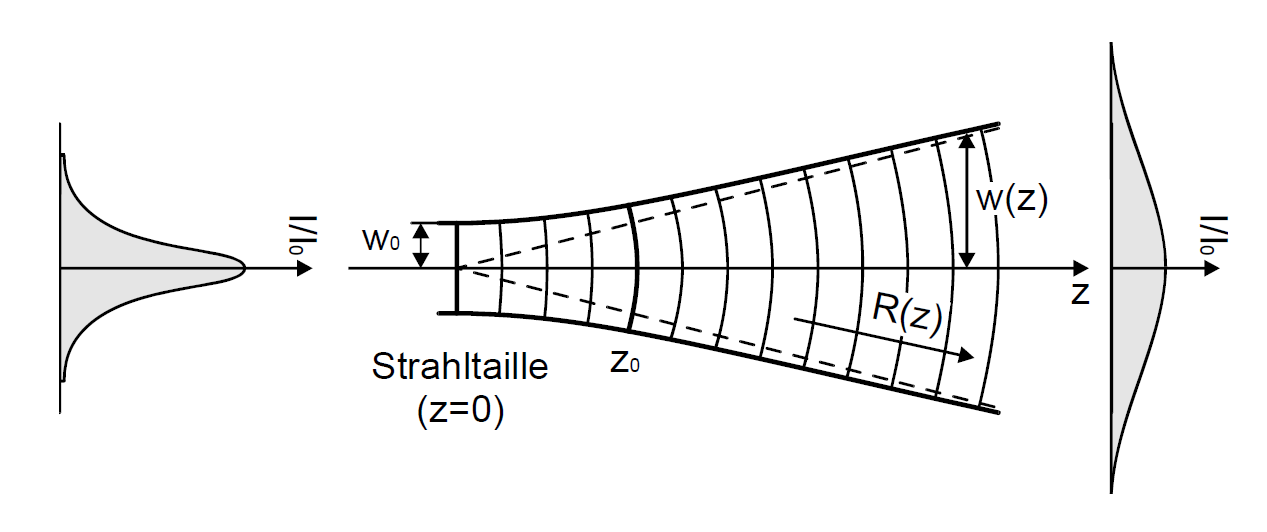
\includegraphics[width=.5\columnwidth]{gauss-strahl.png}
  \caption[Gauss]{Gau\ss{}-Strahl }
  \label{fig:gauss}
\end{figure}

Dieser Strahl wird, wie in~\ref{fig:gauss} ersichtlich, charakterisiert durch
die Strahldicke \(w(z)\) und den Radius der Wellenfronten
\(R(z)\). Die Angabe von Amplitude, Strahltaille \(w(z=0)=w_0\) und
Wellenl\"ange beschreibt den Strahl vollst\"andig.

\subsubsection{Matrizenopik}
\label{sec:matrizen}

Um eine Stabilit\"atsbedingung f\"ur den Resonator aufzustellen, muss
zuerst das Verhalten des Lichtfeldes beschrieben werden. Die
Matrizenmethode der Strahlenoptik ist auch auf Gau\ss{}strahlen
anwendbar und stellt daher ein probates Mittel dar. Diese basiert auf
der zweidimensionalen Darstellung des Lichtstrahles durch einen
Vektor:

\begin{equation}
  \mqty(d \\ \alpha) \widehat{=} \mqty(\text{Abstand zur Achse} \\
  \text{Winkel zur Achse})
\end{equation}

Das optische System wird durch eine Matrix dargestellt, die man
eleganterweise durch Multiplikation der Matrizen der Einzelsysteme
erh\"alt.

\begin{equation}
  \label{eq:systmatrix}
  \mathfrak{M}_{\text{System}}=\mathfrak{M}_{\text{1}}\cdot\ldots\cdot\mathfrak{M}_{n}=\mqty(A
  & B \\ C & D)
\end{equation}

Die hier ben\"otigten Matrizen sind im folgenden aufgef\"uhrt.
{\setlength{\tabcolsep}{20pt}
\begin{table}[h!]
  \centering
  \begin{tabular}{l | c | l}
    \textbf{Element} & \textbf{Matrix} & \textbf{Parameter} \\
    \midrule\\
    \addlinespace[-2ex]
    freie Ausbreitung & \(\begin{pmatrix}
      1 & s \\
      0 & 1
    \end{pmatrix}\) & Wegl\"ange \(s\) \\
    \midrule\\
    \addlinespace[-2ex]
    d\"unne Linse & \(\begin{pmatrix}
      1 & 0 \\
      -1/f & 1
    \end{pmatrix}\) & Brennweite \(f\) \\
    \midrule\\
    \addlinespace[-2ex]
    sph\"arischer Spiegel & \(\begin{pmatrix}
      1 & 0 \\
      -2/R & 1
    \end{pmatrix}\) & Radius \(R\) \\

  \end{tabular}
  \caption{Einige optische Matrizen}
  \label{tab:mats}
\end{table}}

Definiert man einen Parameter
\(\frac{1}{q(z)}=\frac{1}{R(z)}+i\frac{\lambda}{\pi w^2(z)}=a+i\cdot
b\) enth\"alt dieser alle wichtigen Informationen des Strahls in einer
Form, die man mit der Matrizenoptik behandeln kann (sog. komplexer
Strahlradius aus dem Exponenten der mathematischen Darstellung des
Gau\ss{}-Strahls).

So transformiert sich dieser Parameter mit der Matrix
\(\mathfrak{M}_{\text{System}}\) wie folgt:

\begin{equation}
  \label{eq:qtrans}
  q'=\frac{Aq + B}{Cq+D}
\end{equation}

So kann man die Kaustik eines Laserstrahls, der in einem
hemisph\"arischen Resonator entsteht und durch eine Linse mit
Brennweite \(f\) fokussiert wie folgt berechnet.

Da \(R_2=\infty\) kann man \(z=0\) (Postition des Beamwaist) auf die
Spiegelposition legen. Aus dem in~\ref{sec:stabres} diskutierten
Anpassungen, ergibt sich der Beamwaist am Endspiegel zu:

\begin{equation}
  \label{eq:konfwaist}
  w_0^4=\qty(\frac{\lambda}{\pi})^2L(R-L)
\end{equation}

Wenn \(s\) den Weg vor der Linse und \(x\) den Weg nach der Linse
bezeichnet, dann ergibt sich f\"ur den Imagin\"arteil von \(q'\):

\begin{equation}
  \label{eq:qkaust}
  b'=b\cdot\frac{AD-CB}{A^2+B^2b^2}
\end{equation}

Damit kann man den Beamwaist des resultierenden Strahls berechnen:

\begin{equation}
  \label{eq:reswaist}
  w'=\sqrt{\frac{\lambda}{\pi\cdot b'(x)}}
\end{equation}


\subsubsection{Stabilit\"at im Resonator}
\label{sec:stabres}

Wenn man den Gau\ss{}strahl so anpasst, dass \(R(z_1)=R_1,\;
R(z_2)=R_2\) (siehe \ref{fig:gauss-res}) und fordert, dass der Strahl
nach zweifacher Reflexion in sich selbst \"ubergeht, so erhält man ein
geometrisches Kriterium f\"ur die Resonatorstabilit\"at.

\begin{wrapfigure}{r}{10cm}
  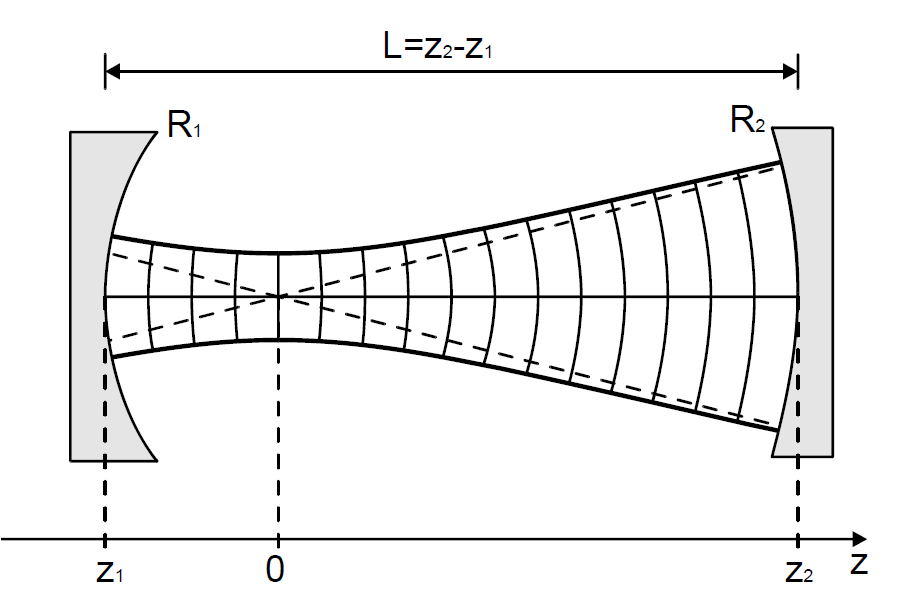
\includegraphics[width=10cm]{gauss-res.png}
  \caption[Gauss]{Gau\ss{}-Strahl im Resonator}
  \label{fig:gauss-res}
\end{wrapfigure}

Mit der Defintion
\begin{equation}
  \label{eq:gparams}
  g_i=1-\frac{L}{R_i};\; i=1,2
\end{equation}

ist ein Resonator stabil, falls:
\begin{equation}
  \label{eq:stabbed}
  0\leq g_1g_2\leq 1
\end{equation}

\subsection{Modenstruktur und Linienverbreiterung des Laser-Lichtes}
\label{ref:linv}

Da, wie in~\ref{sec:reso} diskutiert, mehrere Moden im Resonator
stabil sind, werden im Allgemeinen auch mehrere Moden verst\"arkt.
Unterschiedliche Moden werden in der Regel unterschiedlich
verst\"arkt, sodass nur endlich viele Moden die~\ref{eq:zwlabe}
erf\"ullen, also \"uber der Verlustgrenze liegen.

Da h\"ohere transversale Moden schneller Divergieren als die
Gau\ss{}mode, sind bei diesen Moden die Beugungsverluste gr\"o\ss{}er,
sodass meist nur wenige davon \"uber der Verlustgrenze
liegen.~\cite[171]{Sigrist2018}

Die longitudinalen Moden unterscheiden sich in ihren Frequenzen und
liegen mit steigender Resonatorl\"ange zunehmend dicht
(\ref{eq:longmodes}). Die stimulierte Emission akzeptiert aufgrund der
sog. \textbf{Linienverbreiterung} mehrere Frequenzen, also mehrere
longitudinale Moden, die sich die Besetzungsinversion teilen m\"ussen.

F\"ur die Linienverbreiterung sind unter anderem die Energie-Zeit
Unsch\"arfe, strahlungsfreie \"Uberg\"ange, elastische St\"o\ss{}e
(Druckverbreiterung) und der Dopplereffekt (Dopplerverbreiterung)
verantwortlich. Dabei unterscheidet zwischen \textit{homogener-} (die
ersten drei Beispiele) und \textit{inhomogener} Linienverbreiterung,
wobei erstere auf alle Gassatome gleichzeitig und letztere nur auf
bestimmte Atomgruppen wirkt.

Beim \hne{} in diesem Versuch \"uberwiegt die Dopplerverbreitung,
deren Halbwertsbreite hier angegeben werden soll.

\begin{equation}
  \label{eq:doppler}
  (\Delta\nu)_{\text{Doppler}}=2\cdot \nu_0\qty(\frac{2kT\ln{2}}{mc^2})^{1/2}
\end{equation}

\begin{conditions}
  T & Temperatur \\
  \nu_0 & Zentralfrequenz \\
  m & mittlere Atommasse
\end{conditions}

\subsection{Fabry-Perot-Interferometer}
\label{sec:fabry}

Das \textit{Fabry-Perot-Interferometer} (im Folgenden FPI) beruht auf
Vielstrahlinterferenz, worin sich auch seine hohe spektrale
Aufl\"osung begr\"undet. Die einfallende Welle wird zwischen zwei
planparallelen Fl\"achen (genannt Etalon, Abstand \(d\),
Reflexionsverm\"ogen \(R\)) sehr oft reflektiert. Die Wellen, die das
Etalon verlassen, interferieren nur bei bestimmten Abst\"anden \(d\)
oder Wellenl\"angen \(\lambda\) konstruktiv.

Damit kann das FPI sowohl als Interferometer zur Messung von
Frequenzen, als auch als Modenfilter eingesetzt werden.

Der \textit{freie Spektralbereich} (FSR) des FPI gibt an, wie weit die
einzelnen passierenden Frequenzen auseinander liegen und kann zur
Kalibrierung von Frequenzdifferenzen genutzt werden.
Es gilt:

\begin{eqnarray}
  \label{eq:fsr}
  \text{FSR} = \frac{c}{2\cdot d} = \delta\nu \\
  \Delta\text{FSR} = \frac{c}{2\cdot d^2}\cdot\Delta d
\end{eqnarray}

Die \textit{Finesse} des FPI ist der Quotient aus FSR und
Halbwertsbreite der Peaks, also ein Ma\ss{} f\"ur die Aufl\"osung des
FPI:

\begin{equation}
  \label{eq:finesse}
  \mathfrak{F} = \frac{\pi\sqrt{R}}{1-R}
\end{equation}

Es sollte also \(R\rightarrow 1\) gelten.

Es ist zu beachten, dass die hier aufgef\"uhrten Beziehungen nur bei
senkrechten Strahleinfall gelten.

\subsection{Malus Law}
\label{sec:malus}

Die Intensit\"at einer ebenen Welle nach einem Polfilter ergibt sich
durch Projektion der Eingangswelle auf die Richtung des Filters. Die
Quadratur ergibt sich aus der Intensit\"atsberechnung \(\propto
E^2\). \(\Theta\) bezeichnet den relativen Winkel der
Polarisationsrichtungen.

\begin{equation}
  \label{eq:malus}
  I(\Theta)=I_0\cdot \cos^2{\Theta}
\end{equation}

\section{Versuchaufbau und Ger\"ate}
\label{sec:versuaufb}

Der Versuchaufbau ist schematisch in~\ref{fig:aufb} dargestellt und umfasst unter anderem:

\begin{description}
\item[Spiegel] Nummeriert von 1 bis 10.
\item[Laser] Kommerzieller \hne{} und gr\"uner Justagelaser.
\item[Laserr\"ohre] \hne{} Laserr\"ohre
\item[Blenden] Als Justagehilfe und zum Ausblenden von unerw\"unschten Moden.
\item[Linsen und Filter] Zur Untersuchung der Strahleigenschaften. (Sammellinse, Polfilter, Graufilter)
\item[Fabry Perot Interferometer] Festaufbau, Konfokal
\item[Leistungsmessger\"at] Zur Leistungsmessung und als Justagehilfe.
\item[Faserspektrometer] \textsc{Ocean Optics HR2000+} als Referenzmessger\"at.
\end{description}


\begin{figure}[H]\centering
  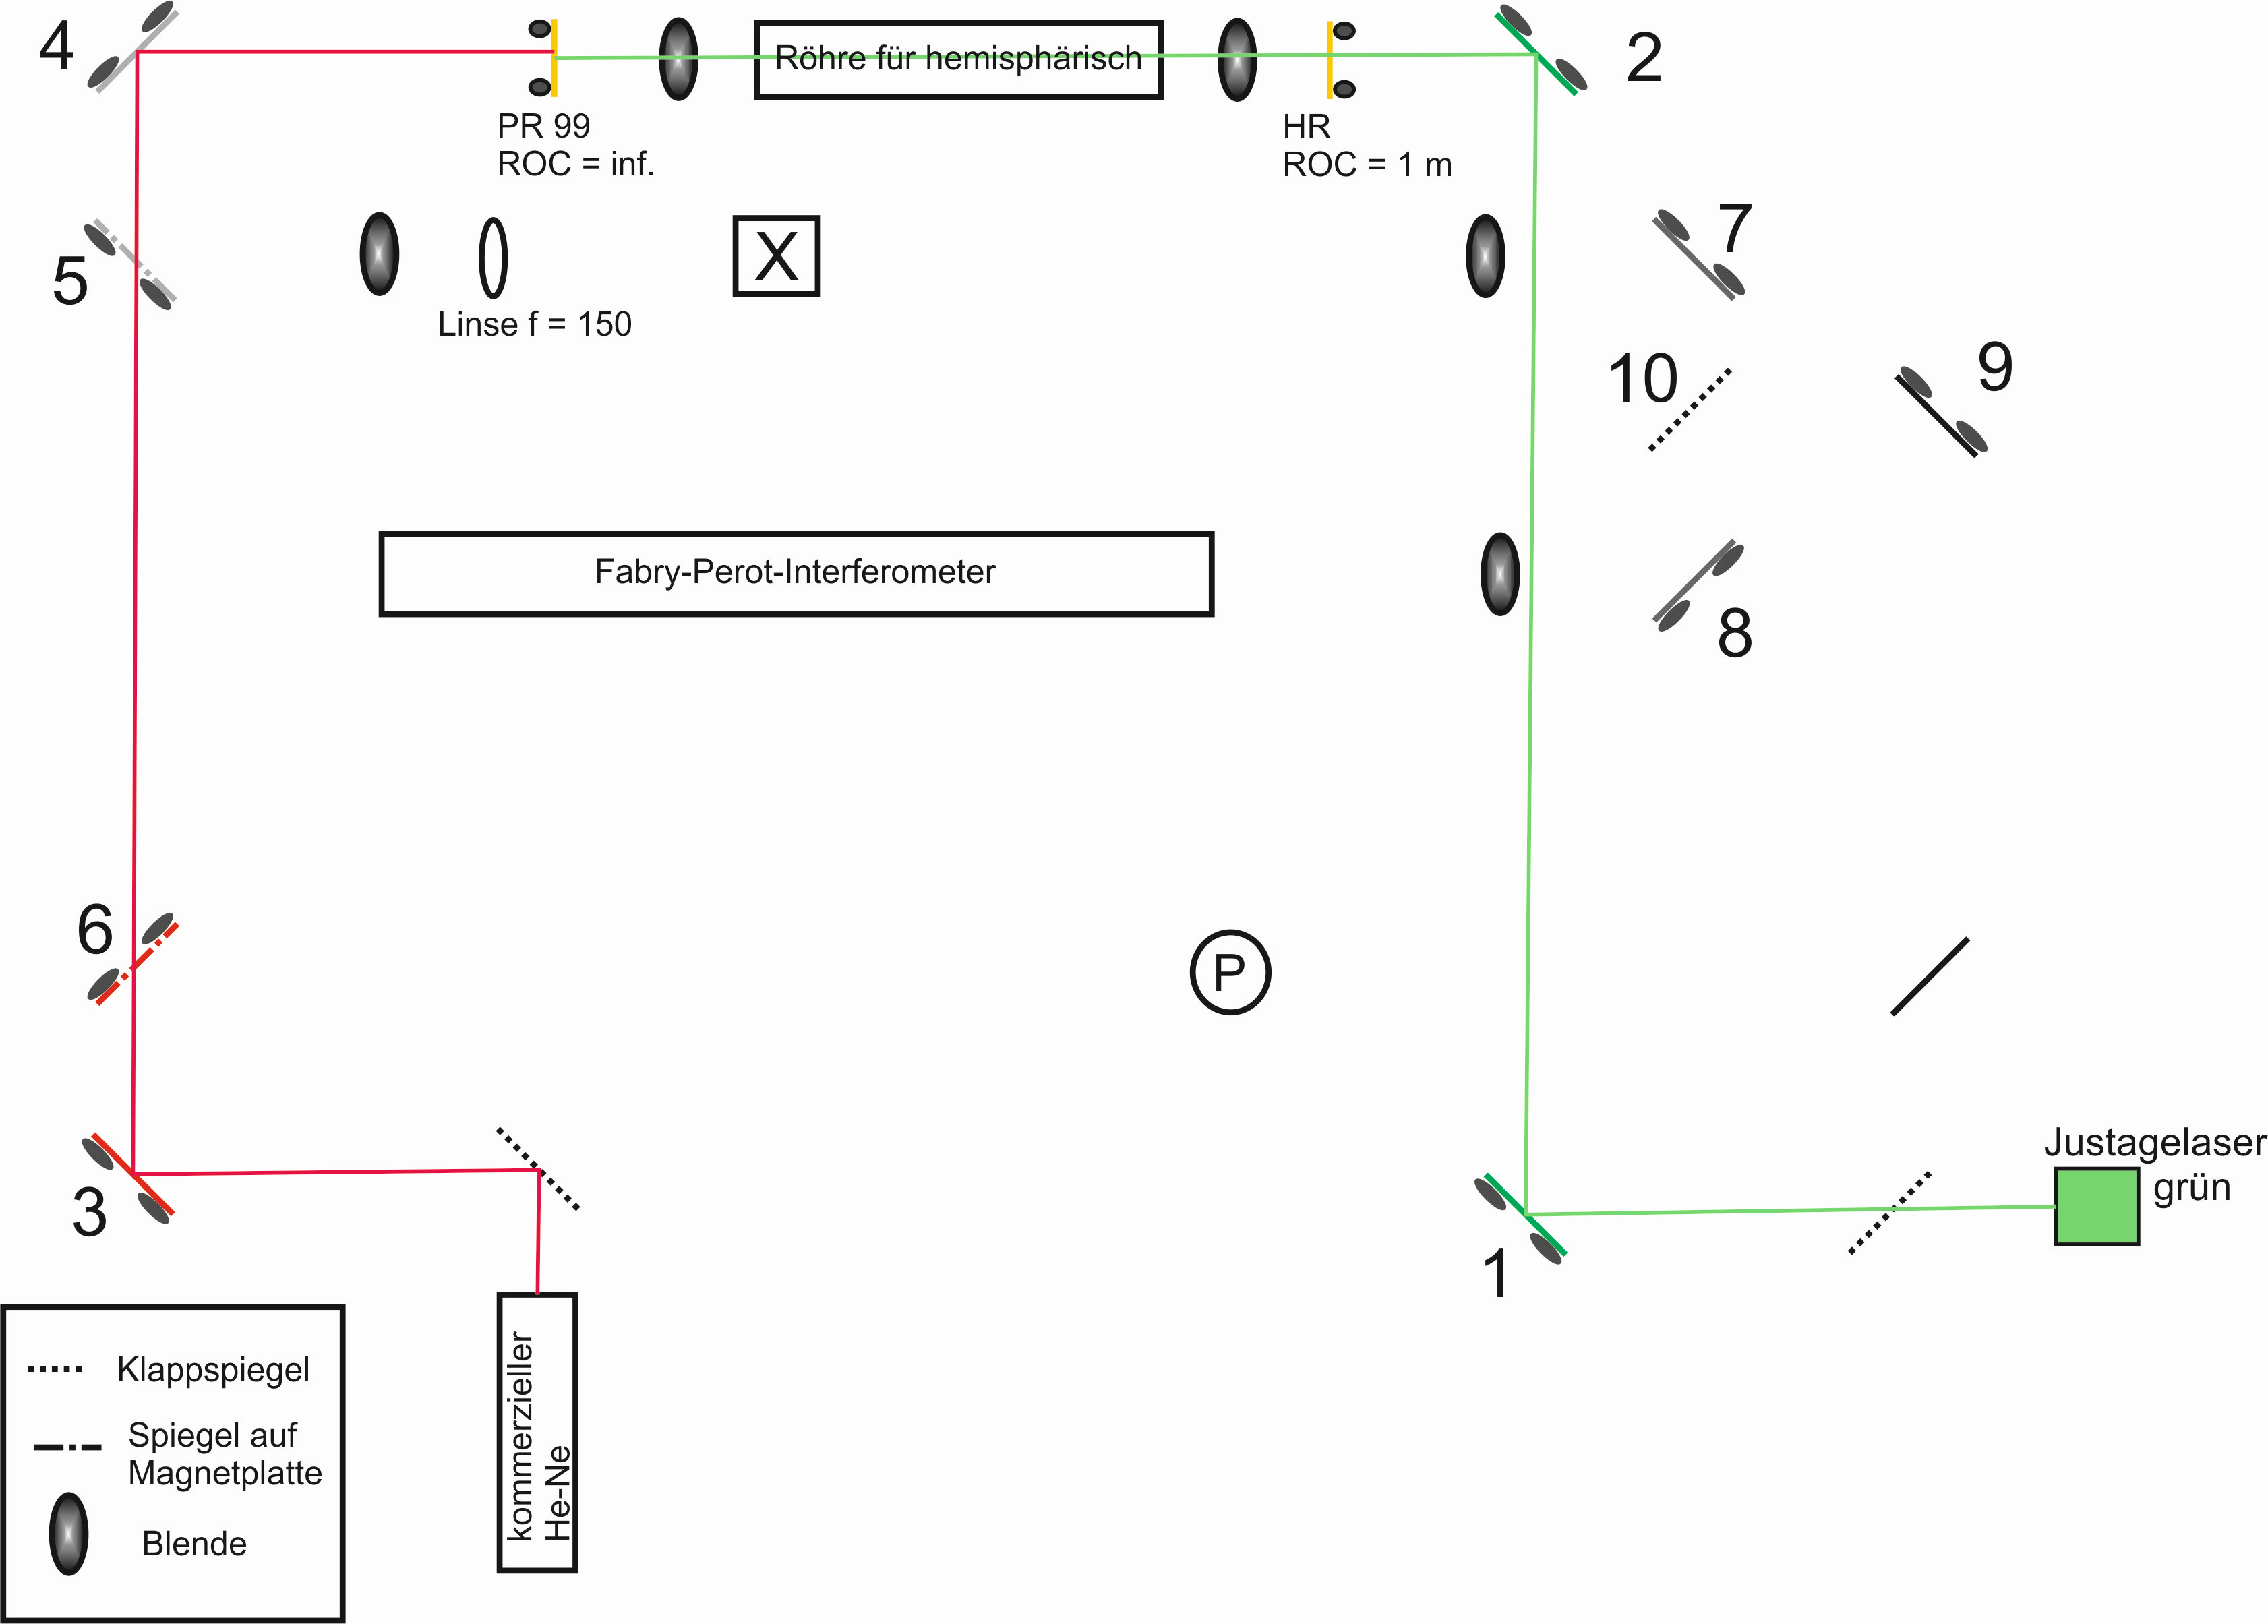
\includegraphics[width=.5\columnwidth]{aufb.png}
  \caption[Aufbau]{Versuchasfbau}
  \label{fig:aufb}
\end{figure}



\section{Durchf\"uhrung}
\label{sec:durch}

\subsection{Stabilit\"atsbereich}
\label{sec:stabber}

Da \(g_1(R_1=\infty)=1\) folgt mit \(R_2=\SI{1}{\meter}\) und \(0\leq
g_2\leq 1\) durch~\ref{eq:stabbed}:

\begin{equation}
  \label{eq:stabber}
  g_2=1-\frac{L}{\SI{1}{\meter}}\implies\SI{0}{\meter}\leq L \leq \SI{1}{\meter}
\end{equation}

Das ist auch aus dem Stabilit\"atsdiagramm ersichtlich. Die orangene
Linie liegt genau f\"ur eben diese \(L\) im Stabilit\"atsbereich.
\begin{figure}[H]\centering
  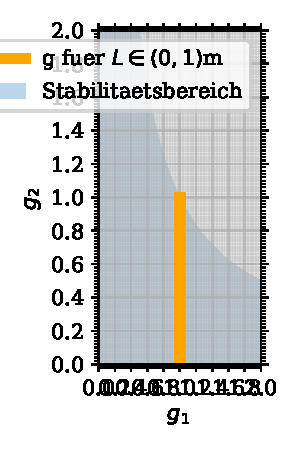
\includegraphics[width=.5\columnwidth]{figs/stabdiag.pdf}
  \caption[Gauss]{Stabilit\"atsdiagramm}
  \label{fig:stabdiag}
\end{figure}

\subsection{Justage und Messung der Verst\"arkung im Einfachdurchgang}
\label{sec:justage}
Ziel des Versuches ist es, in einer mit \hne{} Gemisch gef\"ullte
R\"ohre, einen Laserprozess anzuregen. An dieser R\"ohre sind
Elektroden angebracht, die eine Gasentladung in Gang bringen k\"onnen
(anschalten der R\"ohre). Im ersten Schritt wird daher der
Verst\"arkungseffekt bei Durchgang eines Laserstrahls betrachtet.
Durch Anpassen der Spiegel 4 und 5 und zweier Blenden auf der
optischen Achse (OA) der vormontierten \ce{HeNe}-R\"ohre wurde der
rote Laser parallel zur OA ausgerichtet, sodass er die R\"ohre ohne
st\"orende Reflexe an den Kappilarw\"anden passierte. Auf \"ahnliche
Weise geschah das auch mit dem gr\"unen Laser (\"uber Spiegel 1, 2).

Anschlie\ss{}end wurde die Leistung des kommerziellen Lasers vor der
R\"ohre und bei Durchgang durch diese im deaktivierten und im aktiven
Zustand sowie der Untergrund des Powermeters gemessen. Bei allen
Leistungsmessungen wurde die Raumbeleuchtung abgeschaltet. Die
Messzeit wurde auf \SI{150}{\second} festgelegt, da die Schwankung
des Messwertes ab dieser Zeit annähernd konstant blieb.

\subsection{Aufbau des Hemisph\"arischen Resonators}
\label{sec:aufbauhemi}

Nach dem Einbau der Resonatorspiegel (planar und sph\"arisch) wurde
deren Justage mit Hilfe von R\"uckreflexen der Justagelaser
durchgef\"uhrt. Die anf\"angliche Leistung des Lasers war gering,
konnte jedoch durch Beamwalken (iteratives Feinjustieren der
Stellschrauben an den Spiegel) erheblich gesteigert werden (auf ca
\SI{1}{\milli\watt}).

Anschlie\ss{}end wurde der ausgekoppelte Laserstrahl auf eine zweite
optische Bahn justiert und die Ausgangsleistung des Lasers in
Abh\"angigkeit der Resonatorl\"ange gemessen. Die L\"ange wurde durch
Verschieben des gekr\"ummten Spiegels verstellt.

\subsection{Messung der Polarisationseigenschaften}
\label{sec:poleig}

Nach Einstellung der Resonatorl\"ange auf \SI{80}{\centi\meter}, wurde
ein Polarisationsfilter in den Strahlengang gebracht und die
transmittierte Leistung in Abh\"angigkeit des Polfilterwinkels
gemessen.
Die Messzeit wurde aus Zeitgr\"unden auf \SI{1}{\minute} reduziert.
Da die Polarisationsrichtung des Lasers mit der Nullstellung des
Polfilters \"ubereinstimmte, konnte der Polarisationswinkel absolut
abgelesen werden.

\subsection{Messung der Kaustik}
\label{sec:messkaus}

Zur Messung der Kaustik wurde eine Linse mit \(f=\SI{15}{cm}\)
einem Abstand \(s=\SI{64.5\pm 2.0}{\centi\meter}\) in den Strahlengang
gebracht und alles bis auf die Gau\ss{}mode ausgeblendet. Die
Strahlkaustik konnte dann mit einer CCD Kamera bei fester Linse
aufgenommen werden. Mit dem Programm \textsc{Laser Light Inspector}
wurde nach Anpassung der Belichtung auf eine S\"attigung von
\(200/255\) das FWHM des Laserstrahls durch einen automatischen
Gauß-Fit bestimmt (in vertikaler Richtung, da Anomalie in
horizontaler Richtung). Der Abstand des Kamerasensors wurde durch die
Brennweite der Linse abgesch\"atzt.

Die Messunsicherheiten ergeben sich aus der Schwierigkeit, die genauen
Abst\"ande der Aufpunkte der Spiegel zu bestimmen und wurden
gesch\"atzt.

\subsection{Messung des Spektrums mit dem Faserspektrometer}
\label{sec:faser}

Das Faserspektrometer \textsc{Ocean Optics HR+C1743} wurde in den
Strahlengang gebracht und das Spektrum des offenen \hne{}s digital aufgenommen.

\subsection{Messung von Spektra mit dem FPI}
\label{sec:kalibzeit}

Nach Justage des Strahlengangs auf das FPI durch R\"uckreflexe wurde
der Abstand der Spiegel auf \(d=\SI{7.50+-0.25}{\centi\meter}\)
bestimmt. Dabei war darauf zu achten, dass der Strahl genau mittig auf
die Spiegel trifft, sodass~\ref{eq:fsr} gilt. Falls der Strahl nich in
der Mitte auftrifft kommt es zu Mehrfachuml\"aufen und der
Wegunterschied verdoppelt sich.

Die Ungenauigkeit von \(d\) wurde gesch\"atzt (stat. Ungenauigkeit),
da ein genaues Ablesen wieder aufgrund perspektivischer Effekte
schwierig war.

Anschlie\ss{}end wurde das Spektrum des kommerzielen Lasers ohne
Filter und zweifach mit Polfilter in verschiedenen Stellungen mit Hilfe
eines Digitaloszilloskops aufgenommen. Zwecks der Untersuchung der
longitudinalen Modenstruktur des offenen Lasers wurde dessen Spektrum
bei zwei verschiedenen Resonatorl\"angen gemessen.

\section{Auswertung}
\label{sec:auswertung}

\subsection{Verst\"arkung im Einfachdurchgang}
\label{sec:ausweinf}

\begin{table}[h]
  \begin{tabular}{l|SSSS}
    \toprule
    & {Mittelwert [\si{\micro\watt}]} & {Standartabweichung
                                      [\si{\micro\watt}]} & {Minimum
                                                            [\si{\micro\watt}]}
    & {Maximum [\si{\micro\watt}]} \\
    \midrule
    Untergrund & 0.839 & 0.031 & 0.771 & 0.888 \\
    R\"ohre aktiv & 965.161  & 4.2  & 958.229  & 973.112  \\
    R\"ohre inaktiv & 907.161  & 17.5 & 885.229  & 949.112  \\
    vor R\"ohre & 1319.161 & 2.0  & 1319.229 & 1329.112 \\
    \bottomrule
  \end{tabular}
  \caption{Leistungsmessungen des Einfachdurchgangs mit abgezogenem Untergrund}
  \label{tab:leistungeinfach}
\end{table}

Die systematischen Messungenauigkeiten liegen beim Powermeter weit
unter der statistischen Schwankung und werden hier vernachl\"assigt.

Der Untergrund der Messung ist in Relation zum Rest der Messungen
relativ gering und wurde in~\ref{tab:leistungeinfach} abgezogen. Da
er jedoch eine Gr\"o\ss{}enordnung unter den \"ublichen Messwerten und
deren statistischer Schwankung liegt, wird der Untergrund in allen
folgenden Messungen vernachl\"assigt, weil die Messbereiche nicht
vergleichbar sind.
Die inaktive R\"ohre absorbiert den kommerzielen Laser relativ stark
(ca. \SI{0.4}{\milli\watt}), wobei die Leistung des durch die R\"ohre
transmittierten Strahles relativ stark schwankt.

Die Aktivierung der R\"ohre verst\"arkt den Strahl kaum (\(\approx\)
\SI{6}{\percent}), scheint diesen aber zu stabilisieren, auch wenn die
Leistungschwankung immer noch gr\"o\ss{}er als vor der R\"ohre ist.

Um einen leistungstarken Laser-Strahl zu erzeugen, sind demnach also
viele Durchg\"ange notwendig.

\subsection{Ausgangsleistung in Abh\"angigkeit der Resonatorl\"ange}

Wie in~\ref{fig:power-over-l} zu sehen und in~\ref{tab:leistunglaenge}
zu lesen, bricht die Leistung ab
ca. \SI{90}{\centi\meter} ein und wird bei \SI{1}{\meter} sehr klein.
Das best\"atigt die Stabilit\"atsbedingung aus~\ref{sec:stabber}. Der
Leistungseinbruch vor der eigentlichen Stabilit\"atsgrenze ist
eventuell auf die zunehmende Abweichung von der paraxialen N\"aherung
und Justageschwierigkeiten aufgrund der langen Wegl\"ange
zur\"uckzuf\"uhren.

Die Messabweichungen der L\"ange wurden auf \(\Delta L = \SI{.5}{\centi\meter}\)
abgesch\"atzt und sind von statistischer Natur. Der systematische
Fehler des Lineals ist im Vergleich sehr klein (\(\approx
\SI{.5}{\milli\meter}\)). Der hohe Sch\"atzwert der Messungenauigkeit ist
bedingt druch die Schwierigkeiten des Ablesens der Spiegelposition
(Perspektivabh\"angigkeit durch Abstand zum Ma\ss{}stab).


Vernachl\"assigt wurden hier die Ungenauigkeiten, die sich beim
Einstellen des Leistungsmaximums durch Beamwalken ergeben, da die
Betrachtungen hier eher qualitativer Natur sind.

\begin{figure}[b]\centering
  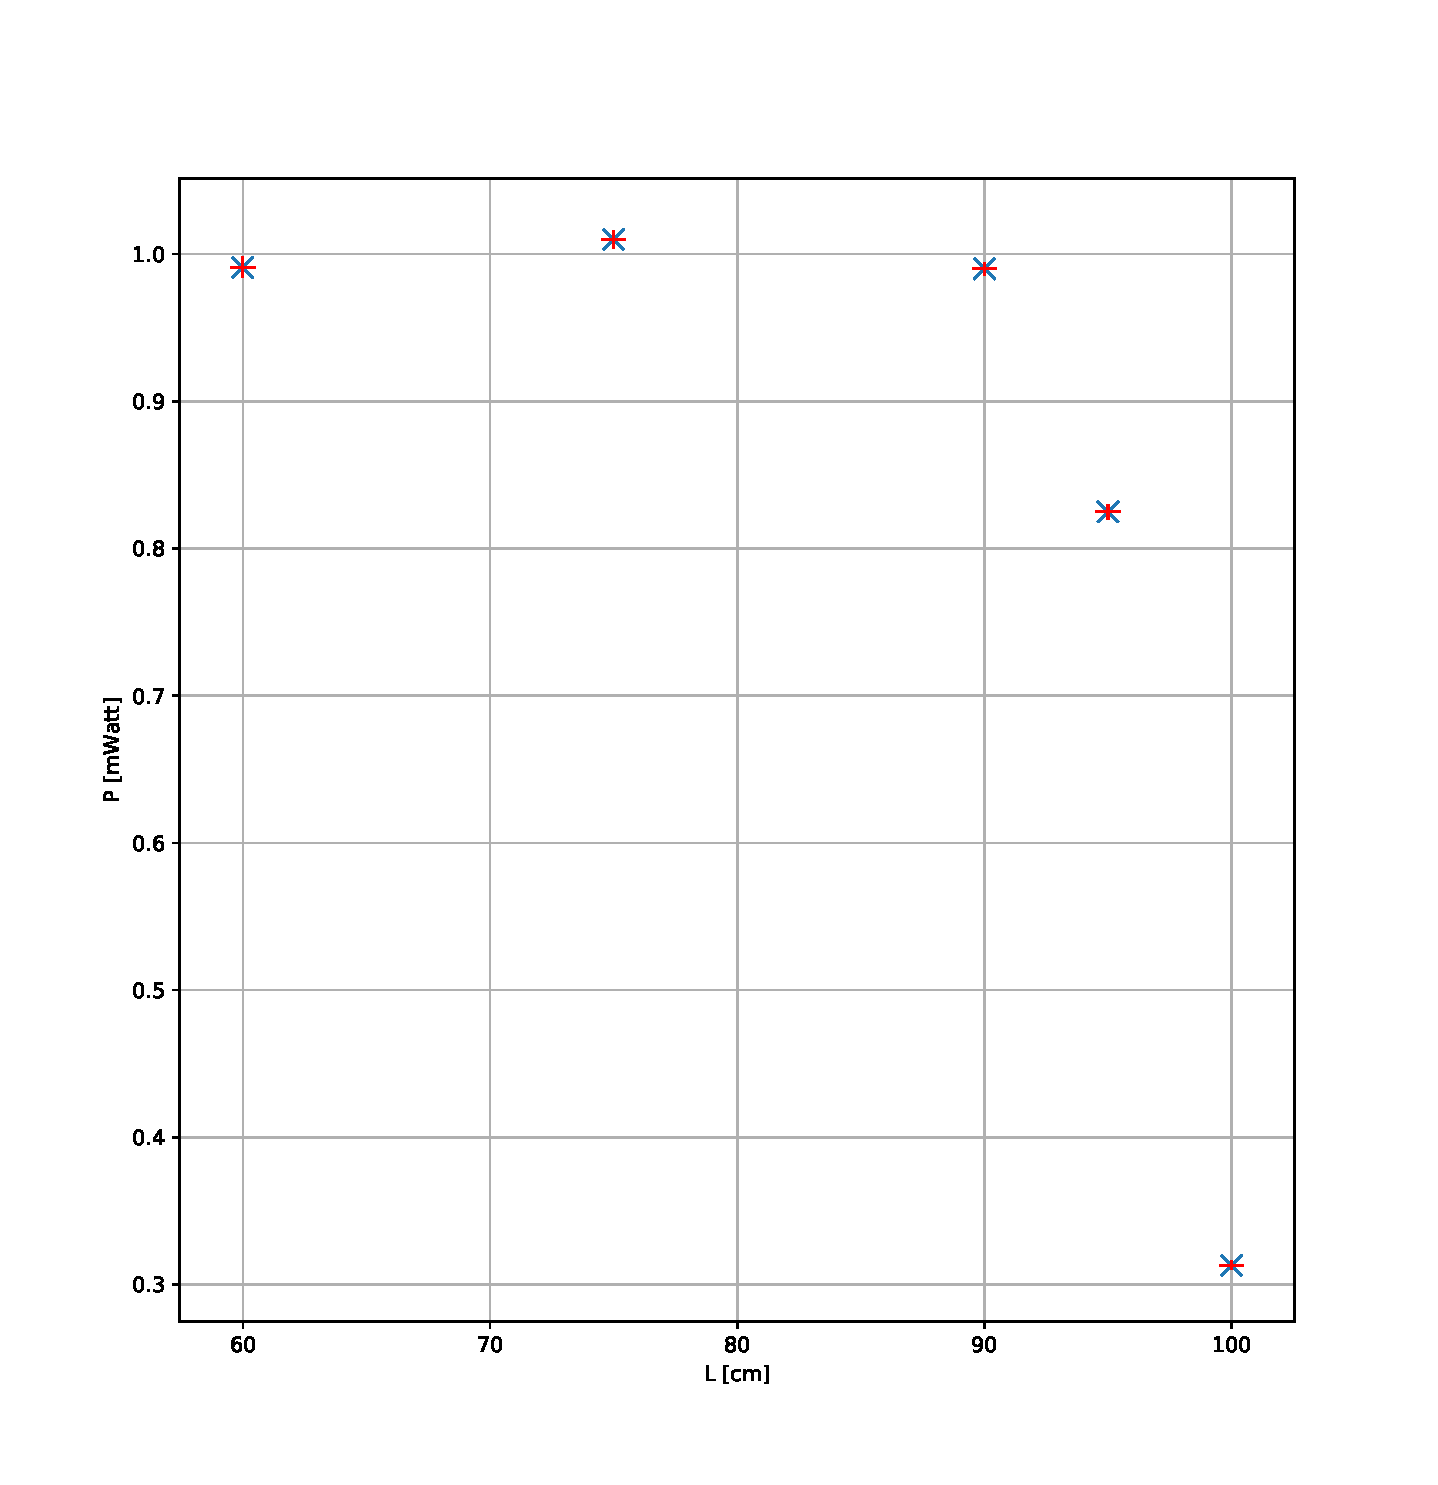
\includegraphics[width=.8\columnwidth]{figs/power-over-l.pdf}
  \caption{Maximale Durchschnittsleistung in Abh\"angigkeit der Resonatorl\"ange }
  \label{fig:power-over-l}
\end{figure}

\begin{table}[b]
  \centering
  \begin{tabular}{SSS}
    \toprule
    {L [\si{\centi\metre}]} & {P [\si{\milli\watt}]} & {\(\Delta\)P [\si{\micro\watt}]}\\
    \midrule
    60  & 0.991 & 7.1  \\
    75  & 1.01  & 6.3  \\
    90  & 0.99  & 4.6  \\
    95  & 0.825 & 3.0  \\
    100 & 0.313 & 5.0  \\
    \bottomrule
  \end{tabular}
  \caption{Maximalleistung in Abh\"angigkeit der Resonatorl\"ange }
  \label{tab:leistunglaenge}
\end{table}

\subsection{Polarisationseigenschaften des Laserstrahls}
\label{sec:diskpol}

Die im Laser verbauten Brewsterfenster erlaubten nur Moden mit einer
Polarisationsrichtung. Alle anderen werden herausreflektiert und
damit nicht verst\"arkt. Somit folgt die Transmission, wie
in~\ref{fig:malus} zu erkennen, sehr gut dem Gesetz von Malus.

Die Messungenauigkeiten resultieren hier aus der Statistik des
Leistungsmessger\"tes und der Einstellung des Polfilters (halbes
Skalenteil \(=0.5^\circ\)), sind also
beide statistischer Natur. Die Abweichungen von der Theorie \"uber die
Abweichungsgrenzen hinaus deuten auf untersch\"atzte (systematsiche)
Faktoren hin.


\begin{figure}[b]\centering
  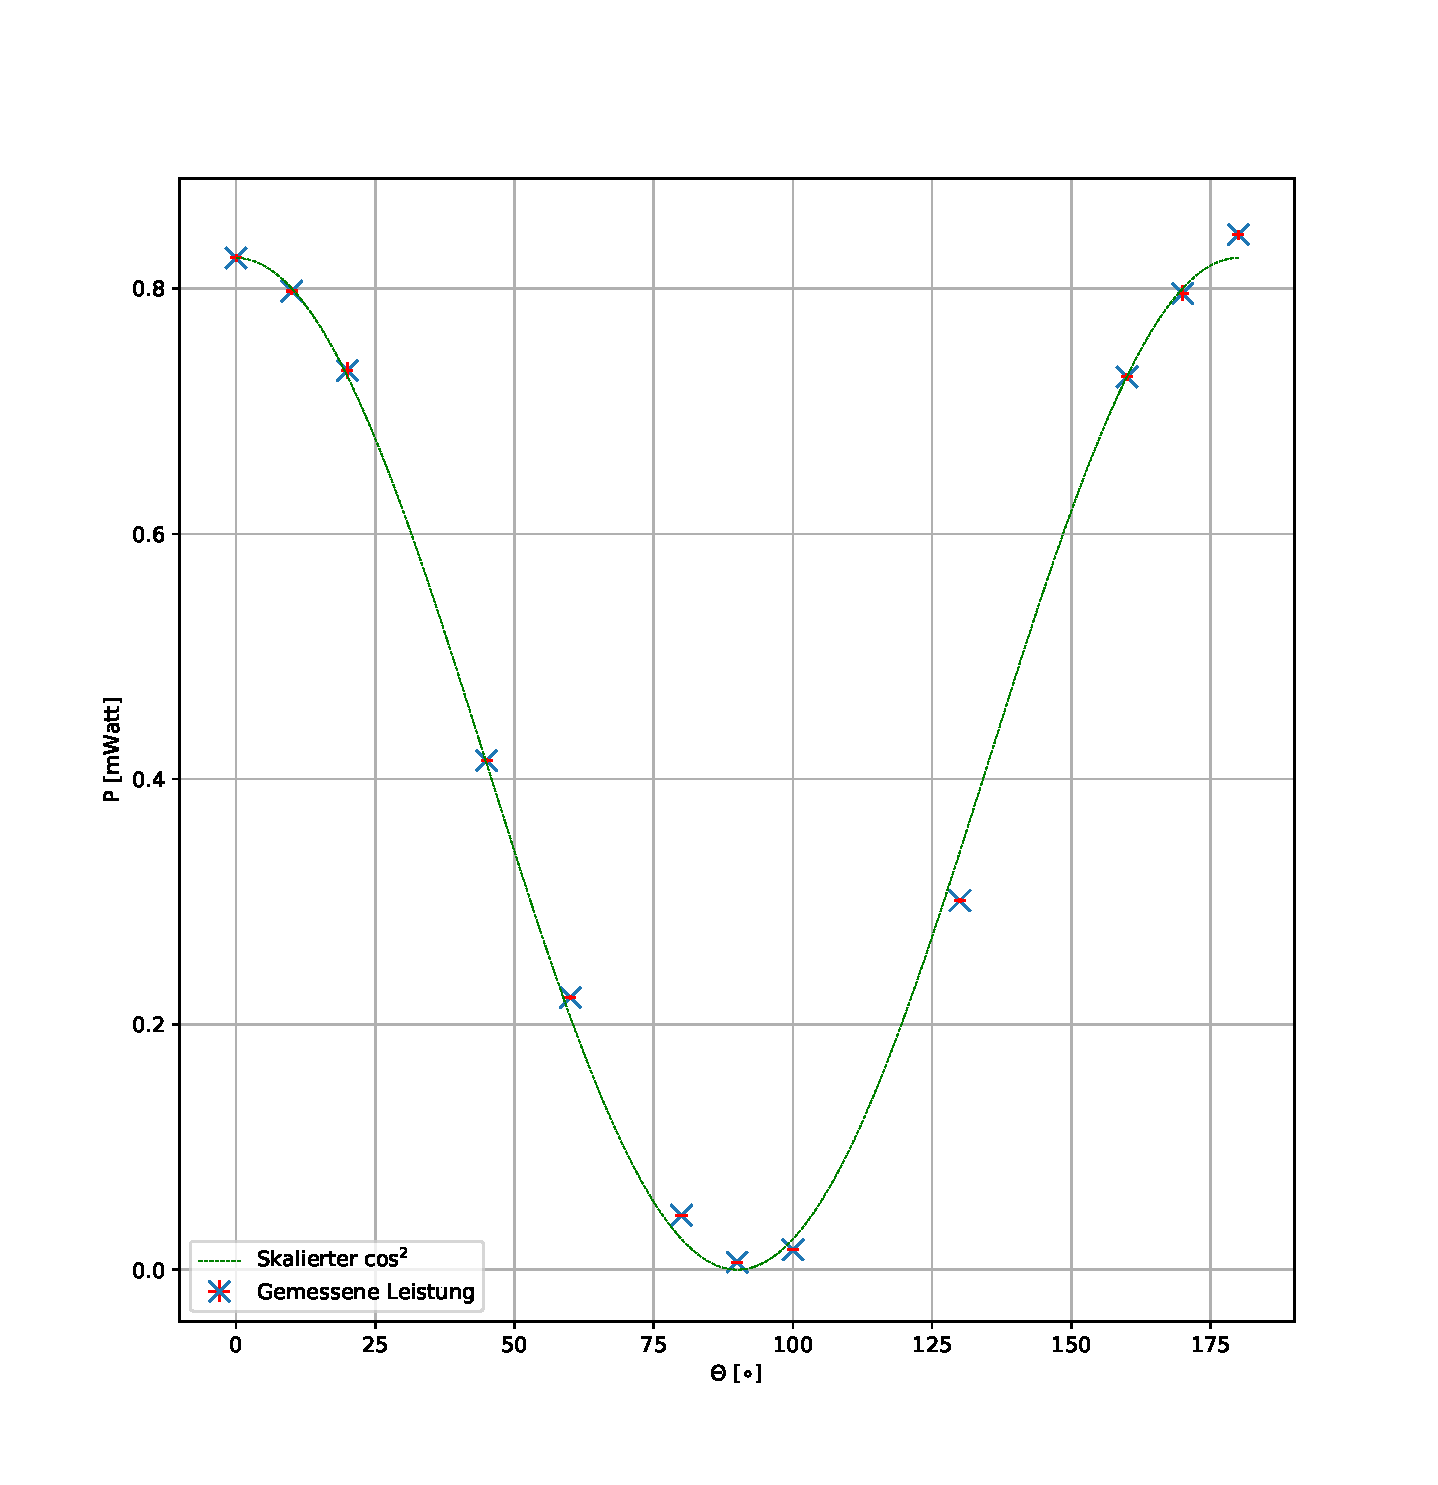
\includegraphics[width=.8\columnwidth]{figs/malus.pdf}
  \caption{Maximale Durchschnittsleistung in Abh\"angigkeit des Polarisationswinkels}
  \label{fig:malus}
\end{figure}

\begin{table}[b]
  \centering
  \begin{tabular}{SSS}
    \toprule
    {\(\Theta\) [\si{\deg}]} & {P [\si{\milli\watt}]} & {\(\Delta\)P [\si{\micro\watt}]}\\
    \midrule
    180 & 0.844   & 3.6     \\
    170 & 0.796   & 6.1     \\
    160 & 0.728   & 3.0     \\
    130 & 0.301   & 1.5     \\
    100 & 0.0163  & 0.084   \\
    90  & 0.00611 & 0.0066  \\
    80  & 0.0445  & 0.22    \\
    60  & 0.222   & 1.7     \\
    45  & 0.415   & 2.2     \\
    20  & 0.733   & 6.7     \\
    10  & 0.798   & 2.7     \\
    0   & 0.825   & 3.1     \\
    \bottomrule
  \end{tabular}
  \caption{Maximale Durchschnittsleistung in Abh\"angigkeit des Polarisationswinkels}
  \label{tab:malus}
\end{table}

\subsection{Messung der Kaustik}
\label{sec:messkaustdisk}
Da die Intensit\"at des Gausstrahls proportional zu
\(\exp{\frac{-2r^2}{w^2}}\) ist, gillt also:

\begin{equation}
  \label{eq:beamwaistfwhm}
  w = 2\sigma = \frac{\overset{\text{der Intensitätsverteilung}}{\text{FWHM)}}}{\sqrt{2\ln{2}}}
\end{equation}

Da die Messung der Entfernung des CCD Chips ungenau war, wurde neben
dem initialen Beamwaist \(w_0\) auch ein Offset \(\delta\) der Kameraposition
gefittet. Es ergeben sich \(w_0=\SI{396\pm 16}{\micro\meter}\) und
\(\delta=\SI{1.2}{cm}\) (Ungenauigkeit aus Fitfehler).

Wie in \ref{fig:kaustik} zu erkennen, ist die \"Ubereinstimmung mit
der theoretischen Kurve sehr gut. Alle Werte stimmen innerhalb der
Toleranzen mit der Theoriekurve \"uberein. Das verifiziert die
Gauß'sche Optik und spricht daf\"ur, dass nur die Gau\ss{}mode angeregt
wurde.

Die Ungenauigkeit der \(z\) Koordinate (Abstand der Kamera) ist
statistischer Natur und wurde auf \SI{1}{\centi\meter} gesch\"atzt
(was sich nun gut mit dem Offset deckt). Die systematsiche
Unsicherheit des FWHM wurde auf \(\SI{1}{px}=\SI{5.6}{\micro\meter}\)
gesch\"atzt.

Der theoretische Wert f\"ur den Beamwaist liegt bei
\SI{284}{\micro\meter} und liegt nicht innerhalb der Toleranzen. Gr\"unde
daf\"ur k\"onnten Effekte an der Blende und Abweichungen der Geometrie
durch ungenaue Einstellung der Resonatorspiegel sein.

\begin{figure}[b]\centering
  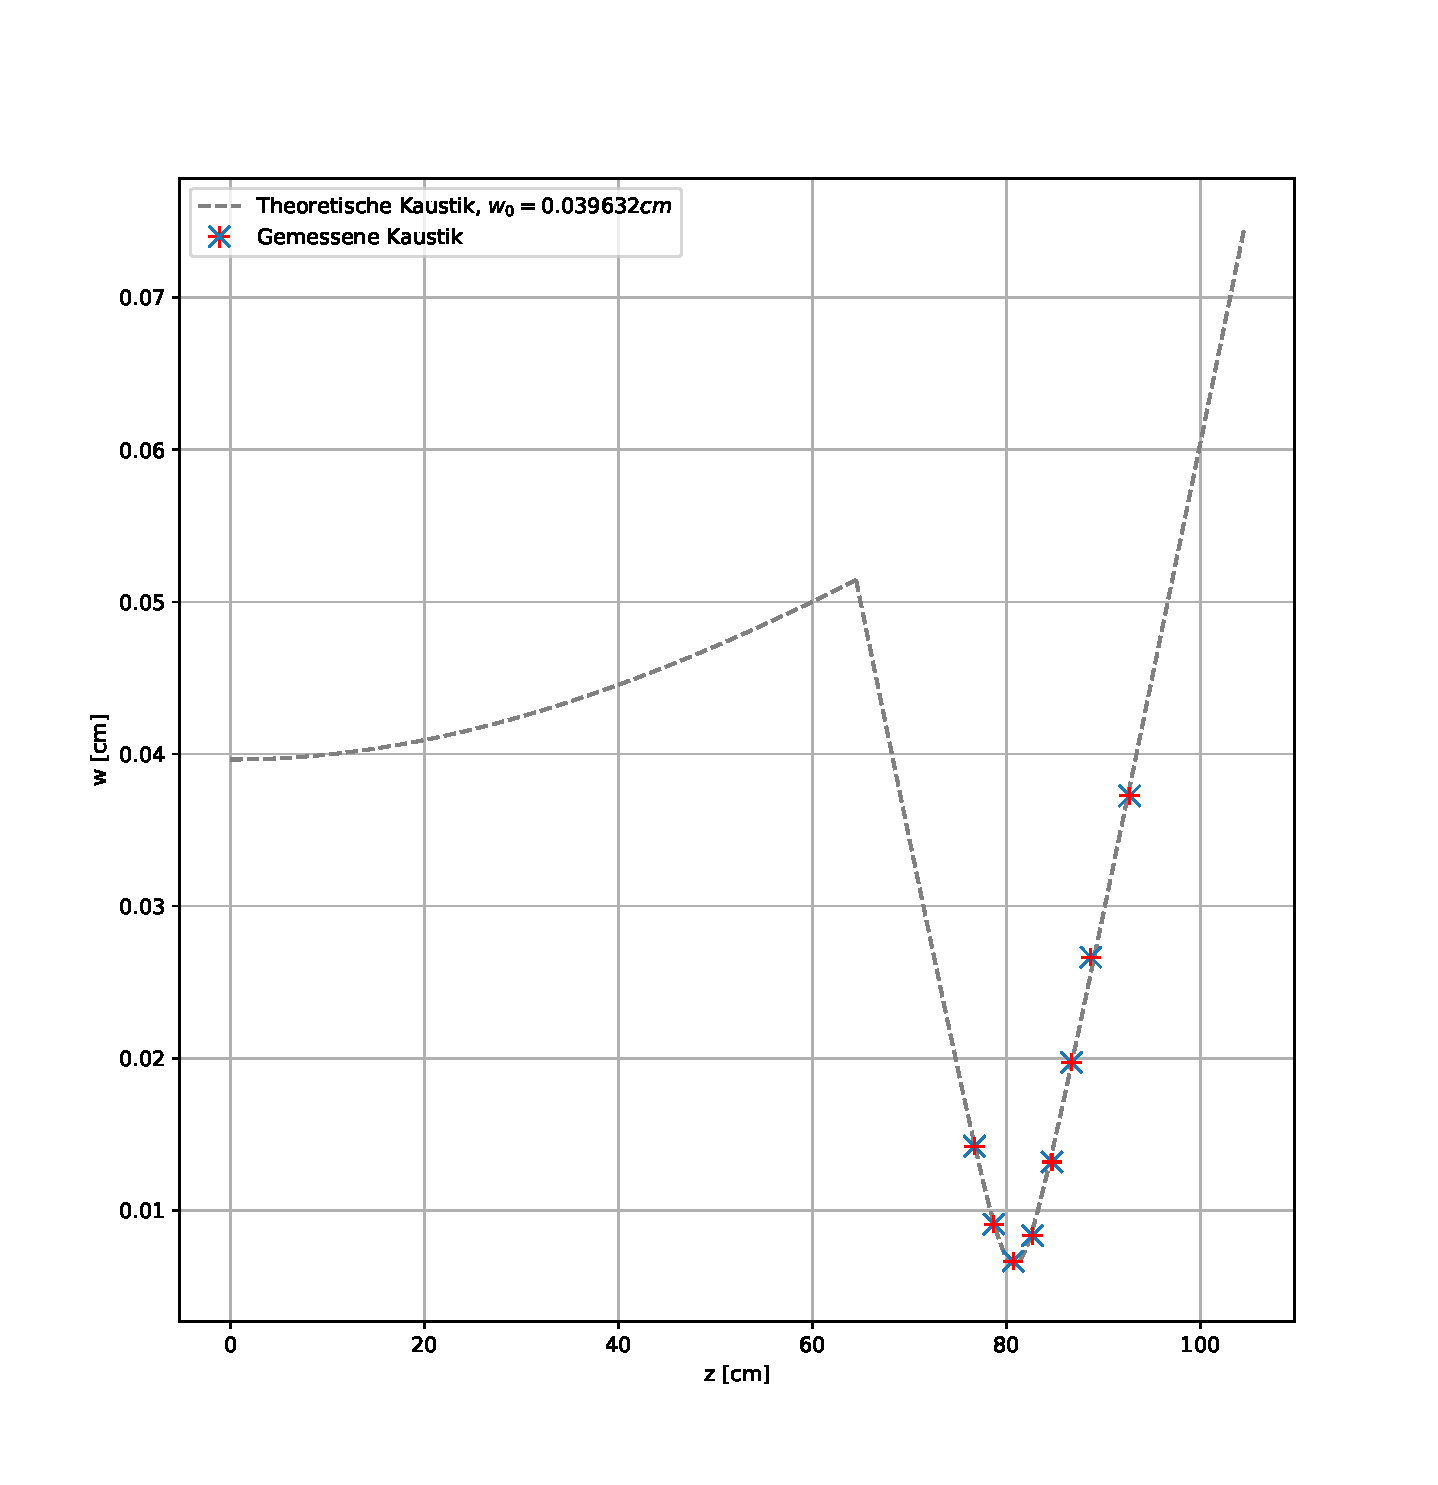
\includegraphics[width=.8\columnwidth]{figs/kaustik.pdf}
  \caption{Gemessene und Theoretische Kaustik}
  \label{fig:kaustik}
\end{figure}

\begin{table}[b]
  \centering
  \begin{tabular}{SSS}
    \toprule
    {\(z\) [\si{\centi\meter}]} & {FWHM [\si{px}]} & {\(w\) [\si{\micro\meter}]}\\
    \midrule
    11 & 29.9 & 142 \\
    13 & 19.1 & 91  \\
    15 & 14.0 & 67  \\
    17 & 17.5 & 83  \\
    19 & 27.7 & 132 \\
    21 & 41.5 & 197 \\
    23 & 56.  & 266 \\
    27 & 78.3 & 372 \\
    \bottomrule
  \end{tabular}
  \caption{Werte der Kaustikmessung}
  \label{tab:kaustik}
\end{table}

\subsection{Messung des Spektrums mit dem Faserspektrometer}
\label{sec:faserausw}

Das in~\ref{fig:faserspek} geplottete Spektrum zeigt, wie zu erwarten
war, einen gro\ss{}en Peak bei
\(\lambda_0=\SI{631.9}{\nano\meter}\). Es sind keine individuellen
Moden erkennbar. Der Abstand der einzelnen Messpunkte betr\"agt rund
\(\Delta\lambda=\SI{.5}{\nano\meter}\).

Damit ergibt sich f\"ur die Frequenzaufl\"osung um \(\lambda_0\):

\begin{equation}
  \Delta\nu=c\cdot\frac{\Delta\lambda}{\lambda_0^2}=\SI{3.30e11}{\hertz}
\end{equation}

Der Modenabstand betr\"agt nach \ref{eq:longmodes} (Ungenauigkeiten
aus \(L=\SI{80+-.5}{\centi\meter}\) erst in vierter Nachkommastelle):

\begin{equation}
  \label{eq:moda}
  \delta\nu = \SI{1.87e8}{\hertz} < \Delta\nu
\end{equation}

Somit k\"onnen keine individuellen Moden aufgel\"ost werden.
\begin{figure}[b]\centering
  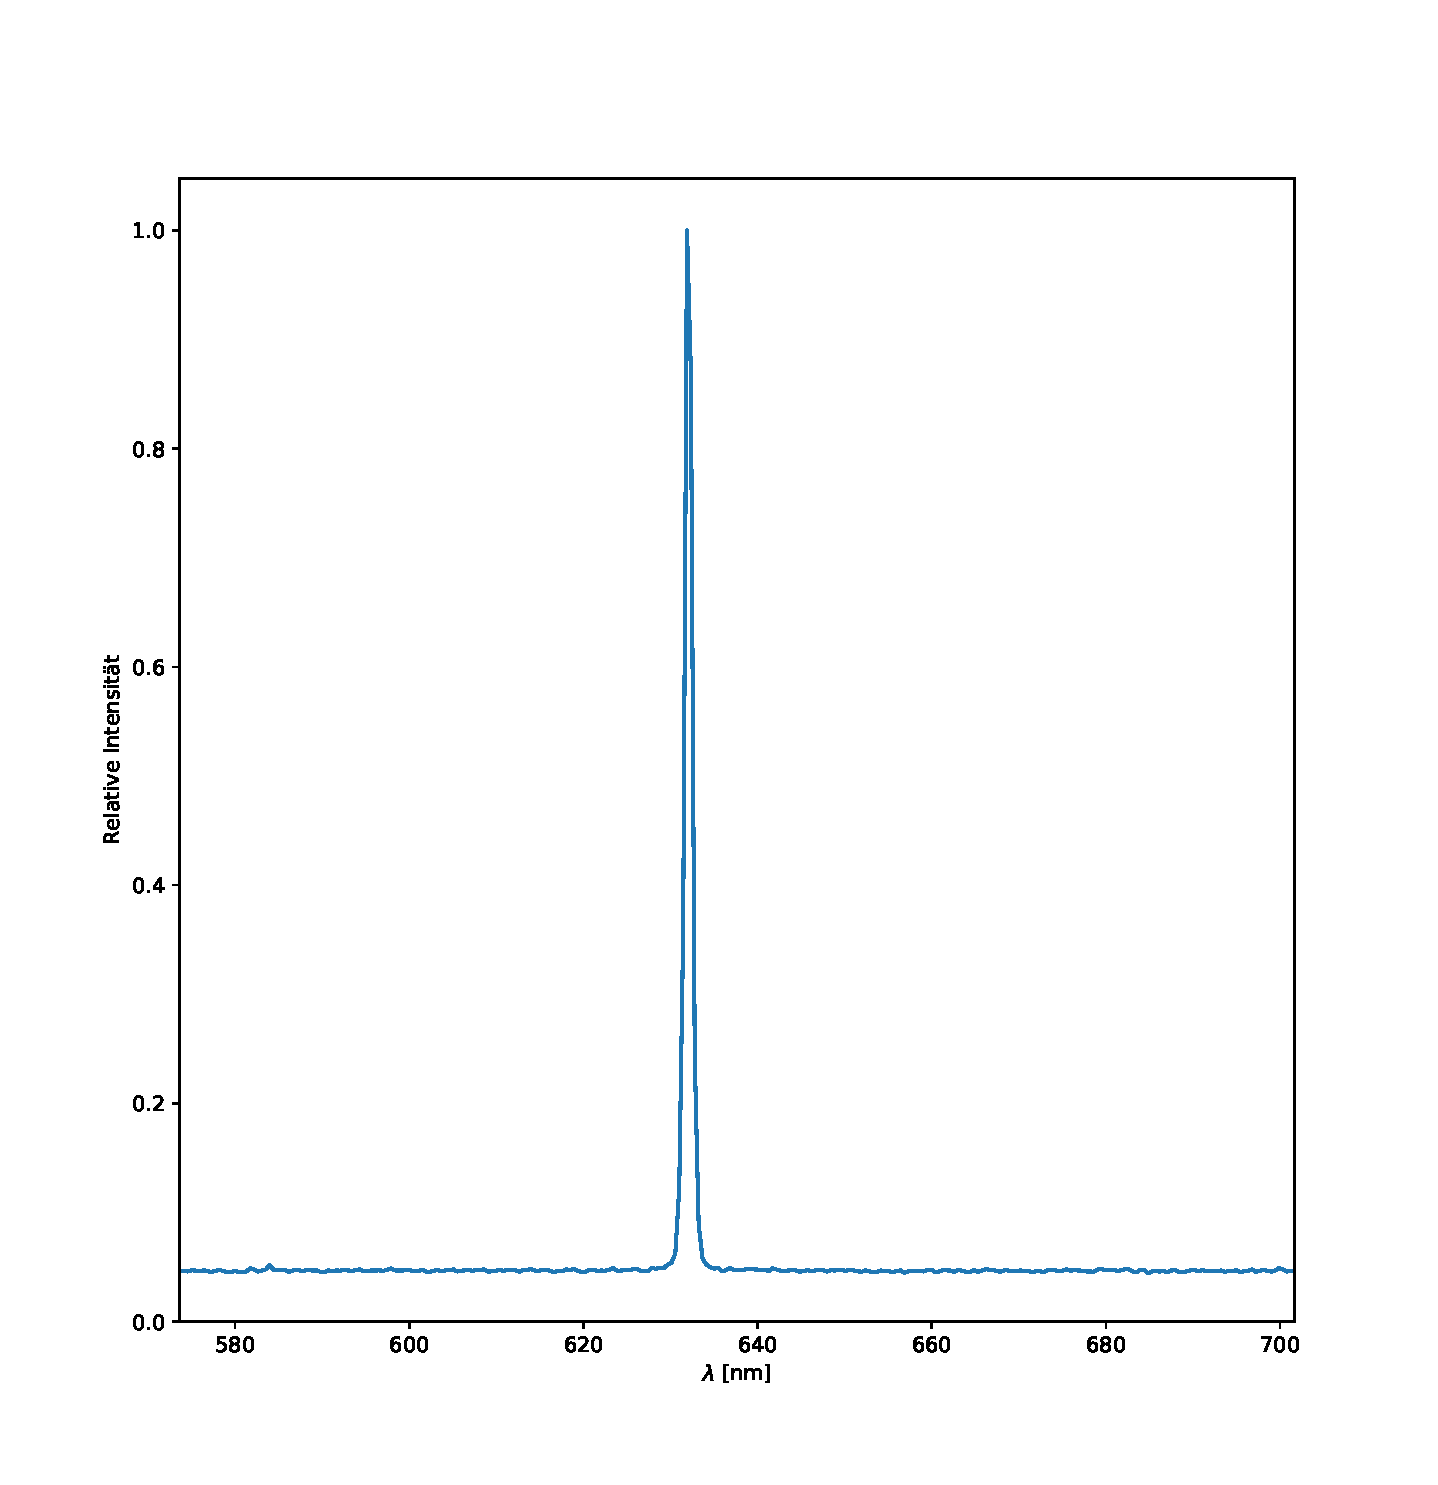
\includegraphics[width=.8\columnwidth]{figs/faserspek.pdf}
  \caption{Spektrum des offenen \hne{}s}
  \label{fig:faserspek}
\end{figure}

\subsection{Kalibierierung der Zeitachse des Oszilloskops}
\label{sec:kalibzeitausw}

Man gewinnt mit~\ref{eq:fsr}:

\begin{equation}
  \label{eq:realfsr}
  \text{FSR} = \SI{2.00+-0.07}{\giga\hertz}
\end{equation}

Im folgenden werden die wird die Einheit der Zeitachse mit \si{u}
bezeichnet. Mit den Positionen zweier zusammengeh\"origer Peaks (siehe~\ref{fig:fsrkalib})
\(t_1=\SI{88}{u},\; t_2=\SI{204}{u}\) (\(\Delta t = \SI{1}{u}\), 1 Digit)
kann man eine Beziehung zwischen \si{u} und \si{\hertz} herstellen.

\begin{eqnarray}
  \label{eq:unithertz}
  \si{u} = \frac{\text{FSR}}{t_2-t_1} =\SI{.172}{\mega\hertz} \\
  \Delta\si{u}  = \sqrt{\qty(\frac{\Delta\text{FSR}}{x_2-x_1})^2 +
  2\cdot\qty(\frac{\text{FSR}}{(x_2-x_1)^2}\Delta t)^2}  & = \SI{.07}{\mega\hertz}
\end{eqnarray}

Die Aufl\"osung des FPI ist also um Gr\"o\ss{}enordnungen besser, als
die des Faserspektrometers.  Die Unsicherheit der Einheitsumrechnung,
die sich aus der L\"angenmessung des FPI und der
Digitalisierungsungenauigkeit fortpflanzt, ist erstaunlich gering.

\begin{figure}[b]\centering
  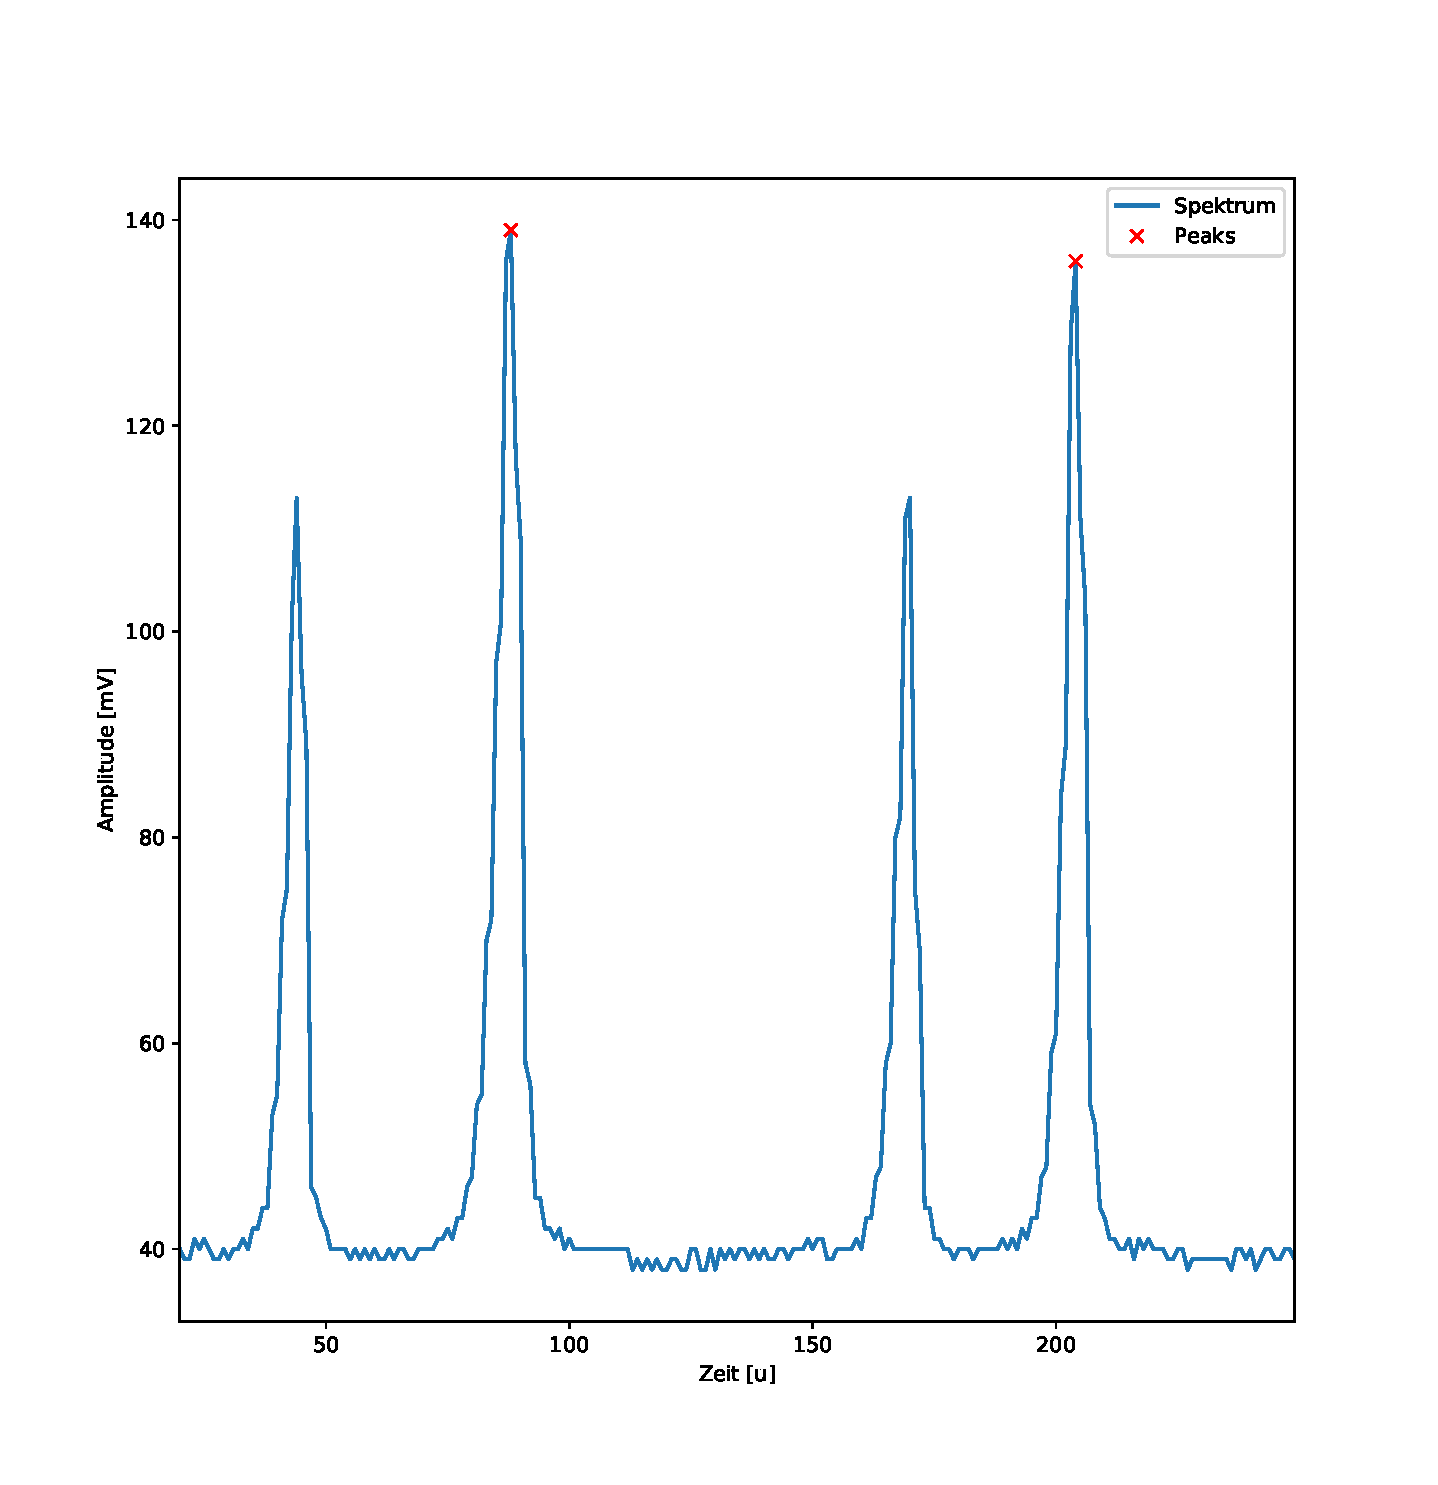
\includegraphics[width=.8\columnwidth]{figs/fsrkalib.pdf}
  \caption{Kalibrierung des FSR, Spektrum des Kommerzielen \hne{}}
  \label{fig:fsrkalib}
\end{figure}

Falls eine Gr\"o\ss{}e \(g\) in \si{u} gemessen und dann in \si{\hertz}
umgerechnet wird, so gilt f\"ur ihre Unsicherheit:

\begin{equation}
  \label{eq:uerr}
  \Delta g = \sqrt{\qty(g\cdot\Delta u)^2 + \qty(\Delta g\cdot u)^2}
\end{equation}

Diese Relation wird im Folgenden immer angewandt.

\subsection{Bestimmung der Finesse}
\label{sec:bestfinesse}

Zur Bestimmung der Finesse wurde das FWHM der vier Peaks
in~\ref{fig:fsrkalib} gemittelt.

\begin{align}
  \label{eq:fwhmlaser}
  \overline{\text{FWHM}} =&\; \SI{4.72}{u} = \SI{81\pm
  6}{\mega\hertz} \\
  \sigma_{\overline{\text{FWHM}}} =&\; \SI{.31}{u}\\
  \Delta\overline{\text{FWHM}} =&
  \sqrt{\qty(\overline{\text{FWHM}}\cdot\Delta u)^2 +
  \qty(\frac{\sigma_{\overline{\text{FWHM}}}}{\sqrt{4}}\cdot u)^2}
\end{align}

F\"ur die Finesse gilt nun:

\begin{align}
  \label{eq:finesselaser}
  \mathfrak{F} =& \frac{\text{FSR}}{\text{FWHM}}=\SI{24.6\pm 2.0}{} \\
  \Delta\mathfrak{F} =&
  \sqrt{\qty(\frac{\Delta\text{FSR}}{\text{FWHM}})^2 + \qty(\frac{\text{FSR}}{\text{FWHM}^2}\cdot\Delta\text{FWHM})^2}
\end{align}

Das ist sicherlich kein überragender Wert (vgl. Anleitung, Anhang),
aber, wie in~\ref{fig:fsrkalib} zu erkennen, zur Aufl\"osung der
longitudinalen Moden ausreichend.

\subsection{Modenstruktur des Kommerziellen Lasers}
\label{sec:modkomm}
Nach~\ref{fig:polarisations} haben die beiden erkennbaren Moden des
kommerziellen Lasers genau orthogonale Polarisation. Ein Plot beider
Spektren in ein Diagramm war leider nicht m\"oglich, da die Daten einer
Aufnahme fehlerhaft waren.


\label{sec:modsturkom}
\begin{figure}[b]\centering
  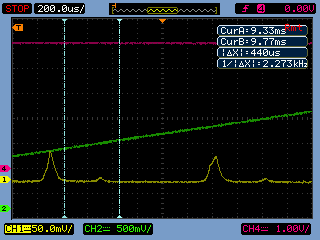
\includegraphics[width=.3\columnwidth]{pol1.png}
  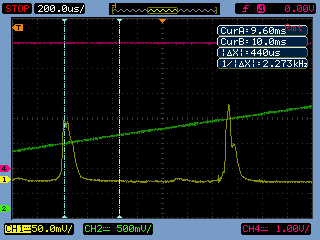
\includegraphics[width=.3\columnwidth]{pol2.png}
  \caption[Gauss]{Spektrum des kommerziellen \hne{}s f\"ur zwei
    orthogonale Polarisationen}
  \label{fig:polarisations}
\end{figure}

Der Abstand der Moden des kommerziellen Lasers wird den Daten
aus~\ref{fig:lengthkomm} entnommen und \"uber die fünf sichtbaren Gruppen
gemittelt:
\begin{figure}[b]\centering
  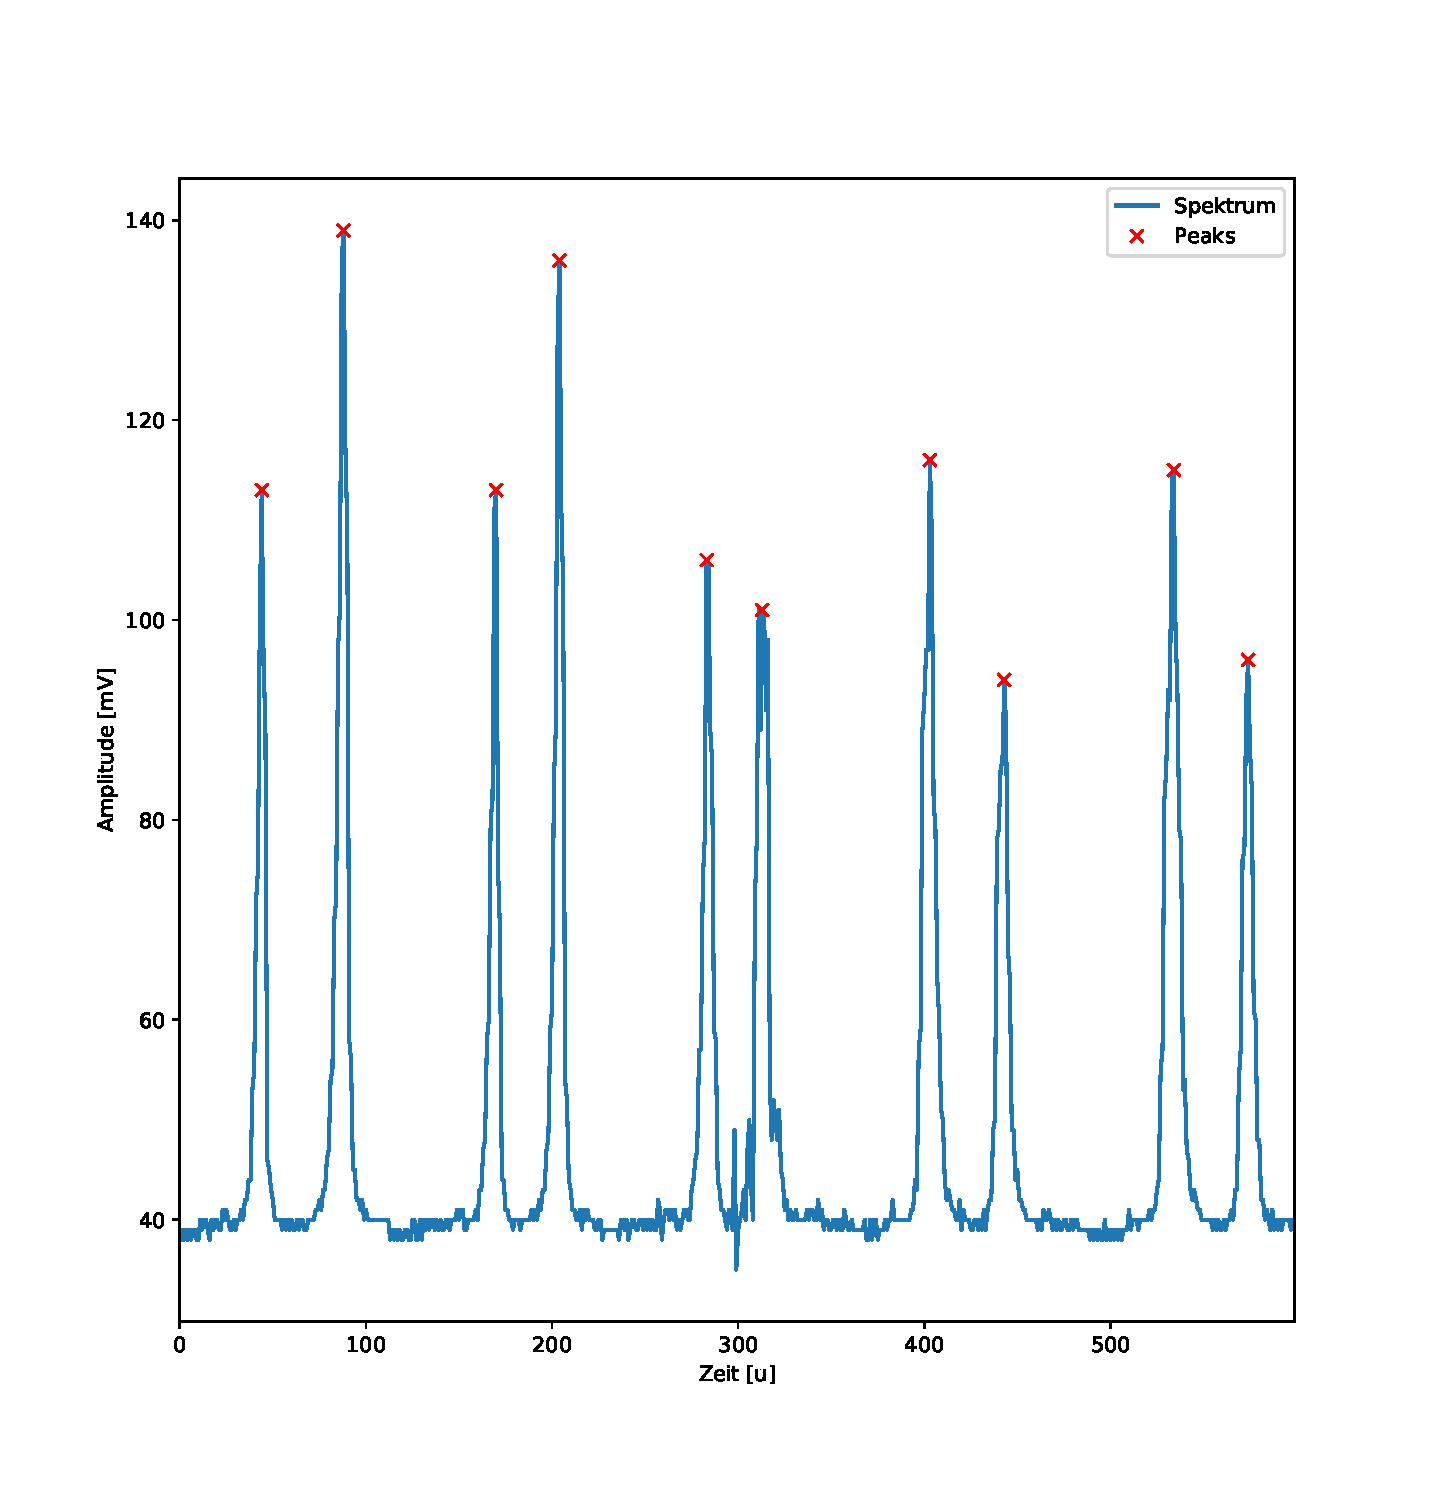
\includegraphics[width=.8\columnwidth]{figs/komm_all_peaks.pdf}
  \caption{Bestimmung der Resonatorl\"ange, Spektrum des kommerziellen \hne{}}
  \label{fig:lengthkomm}
\end{figure}
\begin{equation}
  \label{eq:modeabstkom}
  \overline{\delta\nu_k}=\SI{37.6\pm 2.2}{u}=\SI{650\pm 40}{\mega\hertz}
\end{equation}

Die Ungenauigkeiten kommen hier aus der Statistik der Mittelung.

Damit kann nun die unbekannte L\"ange des Resonators bestimmt werden.

\begin{align}
  L_k =& \frac{c}{2\cdot \delta\nu_k} = \SI{23.1\pm 1.6}{\centi\meter}
  \\
  \Delta L_k =& \abs{\frac{c}{2\cdot\delta\nu_k^2}\cdot \Delta\delta\nu_k}
\end{align}

Dieses Ergebnis erscheint plausibel und die Pr\"azision ist mit den
vorhergehenden L\"angenmessungen vergleichbar.

\subsection{Longitudinale Modenstruktur des offenen \hne{}}
\label{sec:longoff}

Die Bestimmung des Modenabstandes verl\"auft analog
zu~\ref{sec:modkomm} (auch hier wird gemittelt).  Da sich der Maßstab
der Zeitachse des Oszilloskops ge\"andert hat, muss die Umrechnung in
\si{\hertz} wieder analog zu~\ref{sec:kalibzeitausw} kalibriert
werden.

Die gemessenen Spektren und Peakpositionen sind in~\ref{fig:off_80_60} dargestellt.
\begin{figure}[b]\centering
  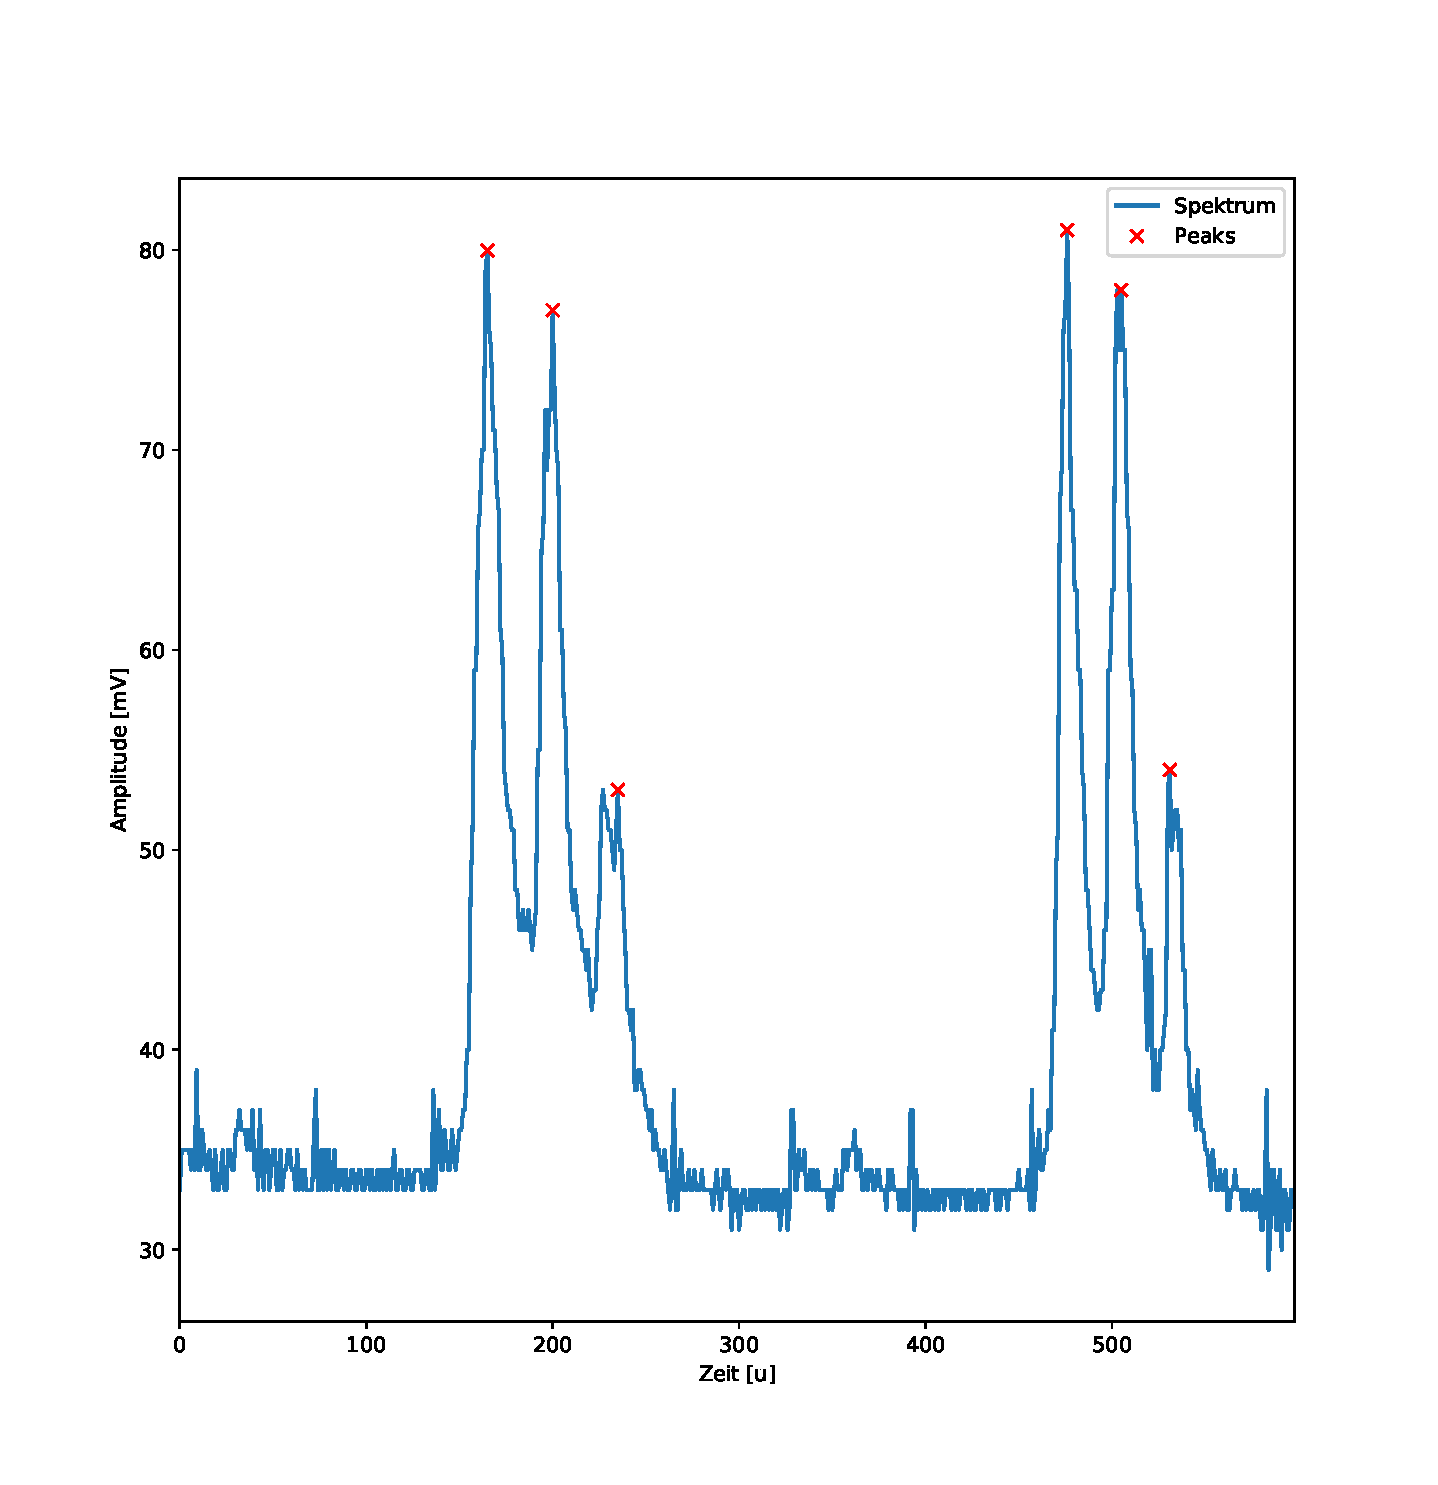
\includegraphics[width=.5\columnwidth]{figs/off_80.pdf}
  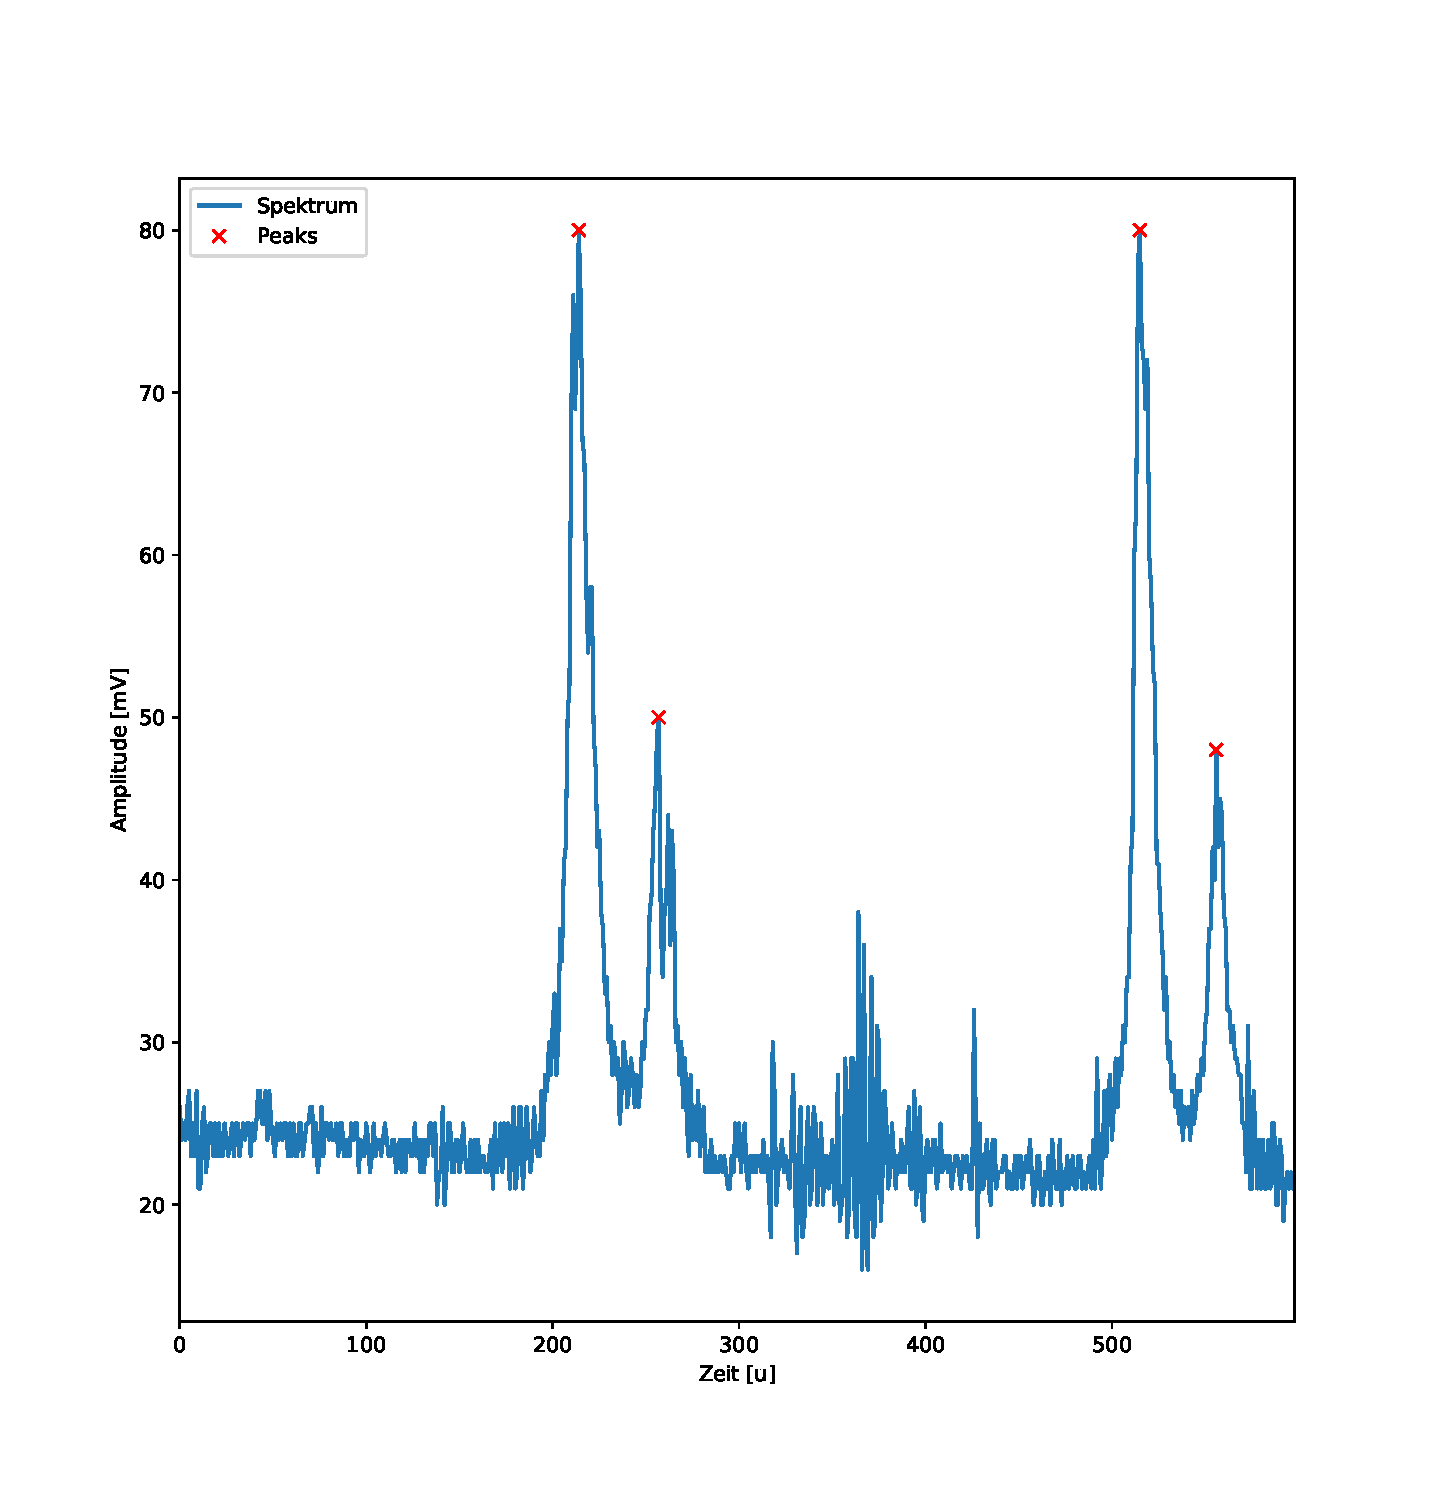
\includegraphics[width=.5\columnwidth]{figs/off_60.pdf}

  \caption{Spektrum des offenen \hne{} bei \(L=\SI{80}{\centi\meter}\)
  und \(L=\SI{60}{\centi\meter}\)}
  \label{fig:off_80_60}
\end{figure}

Die Pr\"azision ist hier durch die geringe Anzahl von sichtbaren Moden
limitiert.

Die Ungenauigkeit der Messung der Resonatorl\"ange wurde wieder auf
\SI{.5}{\centi\meter} gesch\"atzt.

Mit~\ref{eq:longmodes} kann aus der Resonatorl\"ange der Modenabstand berechnet
werden. Man erh\"alt nun f\"ur die Modenabst\"ande:

\begin{table}[H]
  \centering
  \begin{tabular}{SSS}
    \toprule
    {\(L\) [\si{\centi\meter}]} & {\(\delta\nu\) Theorie [\si{\mega\hertz}]} & {\(\delta\nu\) experimentell [\si{\mega\hertz}]}\\
    \midrule
    80 & 187.4\pm 1.2 & 201\pm 14 \\
    60 & 249.8\pm 2.1 & 279\pm 11 \\
    \bottomrule
  \end{tabular}
  \caption{Modenabs\"ande am offenen \hne{}}
  \label{tab:longmodstruk}
\end{table}

Es ergibt sich also f\"ur \(L=\SI{60}{\centi\meter}\) in
\"Ubereinstimmung innerhalb der Fehlergrenzen. F\"ur
\(L=\SI{60}{\centi\meter}\) ist die Differenz gr\"o\ss{}er als die
Messungenauigkeiten. Dieser Umstand k\"onnte eventuell auf die geringe
Anzahl von Peaks \"uber die gemittelt wird zur\"uckzuf\"uhren sein. Da
somit die Statistik mangelhaft wird, k\"onnten vernachl\"assigte
systematische Abweichungen zum Tragen kommen (die Messunsicherheiten
wurden untersch\"atzt).

\subsection{Betrachtung der Linienverbreiterung}
\label{sec:linver}

Die geringe Anzahl sichtbarer Moden macht es schwierig, qualifizierte
Aussagen \"uber die Einh\"ullende zu treffen und l\"asst auf eine hohe Verlustgrenze
schlie\ss{}en. Eventuell wurde auch die zum Ausblenden der
ungew\"unschten Transversalmoden verwendete Blende zu sehr zugedreht.

Die Temperatur in der Laserr\"ohre sollte die Umgebungstemperatur
\(\approx \SI{300}{\kelvin}\) \"ubersteigen. Wie in der Anleitung und
in~\cite[60]{Sigrist2018} dargestellt, sollte bei solchen Temperaturen
der Hauptanteil der Linienverbreiterung durch die inhomogene
Dopplerverbreiterung zustandekommen (Dopplerverbreiterung
ca. \SI{1.5}{\giga\hertz}). Die Einh\"ullende des Modenspektrums
sollte also einer Gaußkurve gleichen, da die Intensit\"aten der
einzelnen Moden zum Profil der Dopplerverbreiterung proportional sind
(Gau\ss{}kurve).

Um eine Schätzung f\"ur die Linienverbreiterung zu erhalten, wurde
eine Gaußfunktion \"uber die drei bei \(L=\SI{80}{\centi\meter}\)
sichtbaren Peaks mit abgezogener Baseline gefittet
(siehe~\ref{fig:fit_einh}). Als freie Parameter wurden die
Standardabweichung \(\sigma\) und die H\"ohe gew\"ahlt. Der
Mittelwert wurde fest auf den h\"ochsten Peak gelegt, da die
Verst\"arkung im Zentrum des Verbreiterungsprofils am gr\"o\ss{}ten
ist.

\begin{figure}[b]\centering
  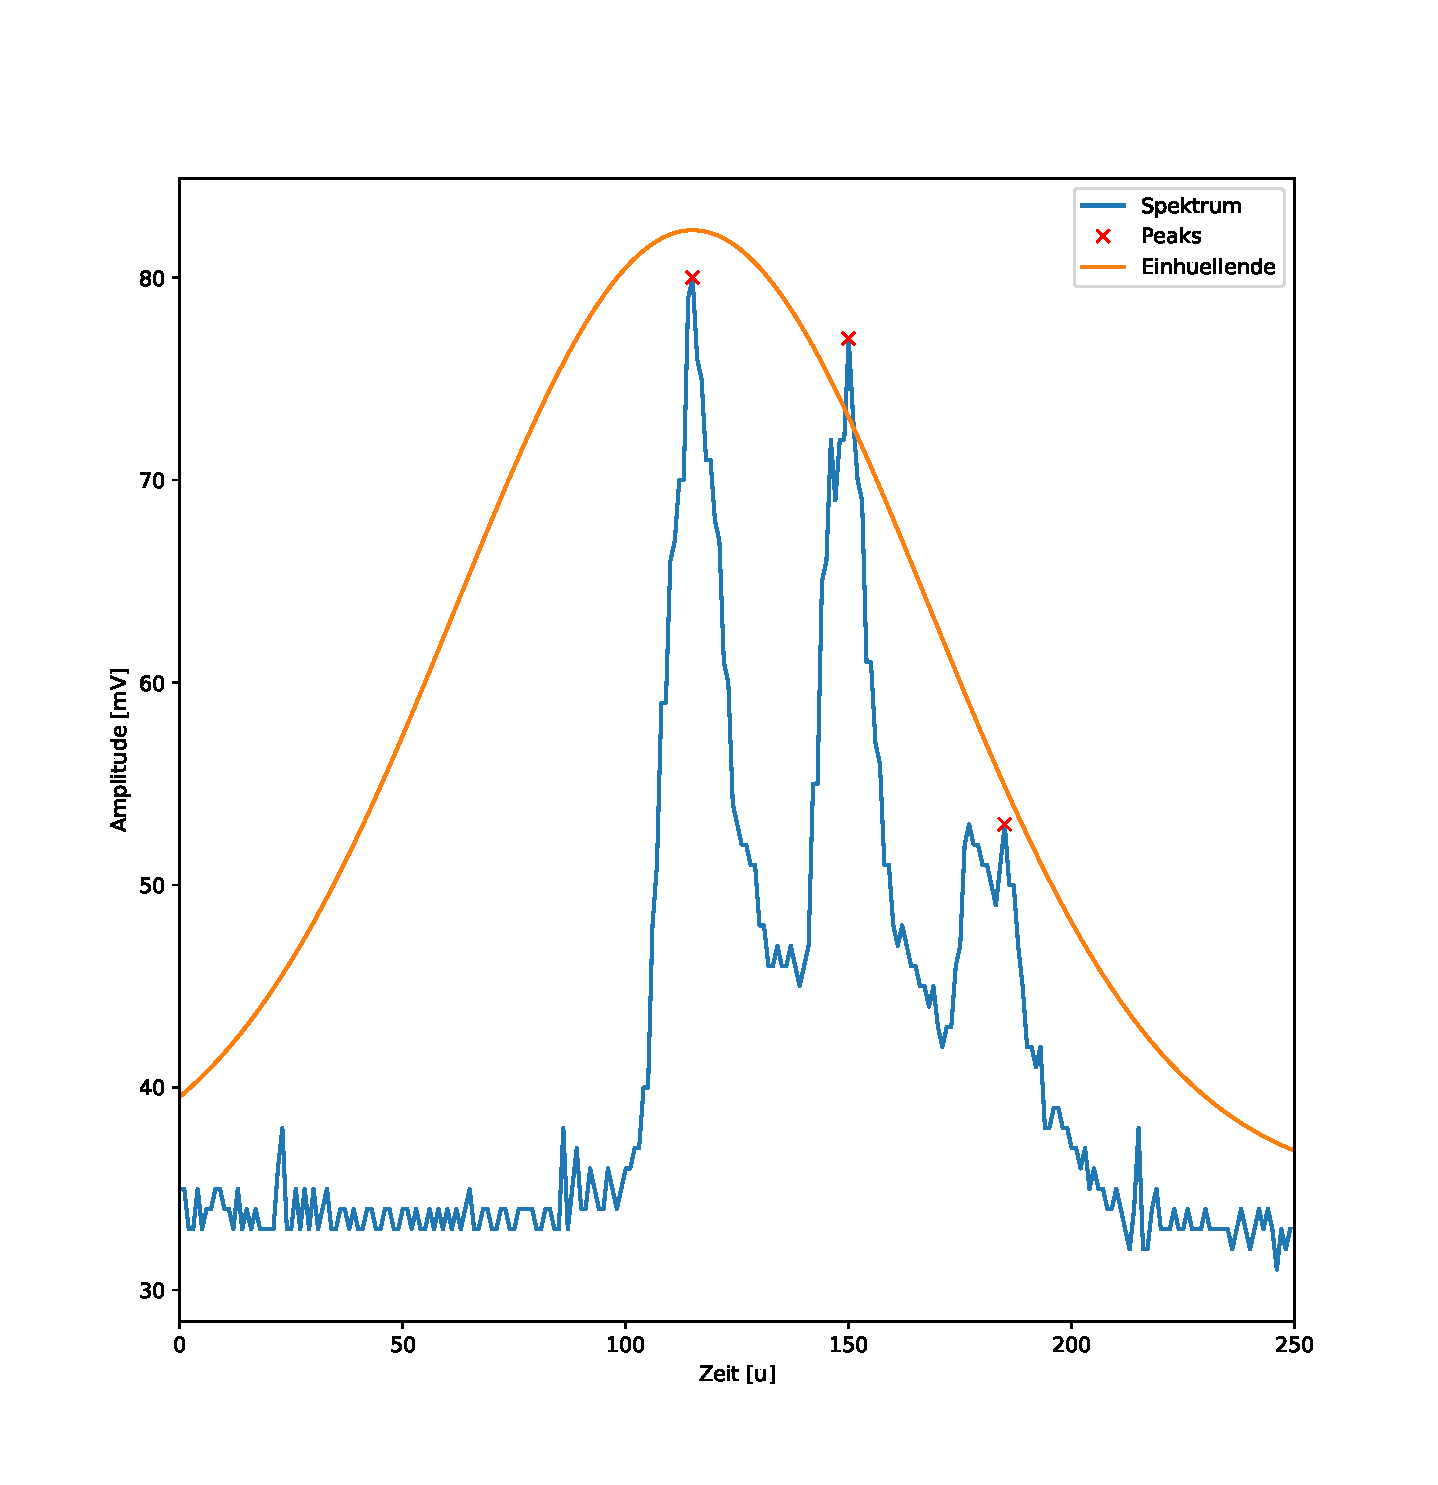
\includegraphics[width=.8\columnwidth]{figs/verbr_fit.pdf}

  \caption{Einh\"ullende der Intesit\"aten der longitudinalen Moden
    des offenen \hne{}}
  \label{fig:fit_einh}
\end{figure}

F\"ur die Standardabweichung und Breite ergibt sich nun:

\begin{align}
  \sigma =& \SI{53\pm 20}{u} = \SI{340\pm 130}{\mega\hertz} \\
  \Delta\nu =& 2\sqrt{2\ln{2}}\cdot\sigma = \SI{800\pm 300}{\mega\hertz}
\end{align}

Die Abweichung von \(\sigma\) ergibt sich nicht aus dem Fit Residuum,
sondern wurde gesch\"atzt. Die erhaltene Linienverbreiterung
\(\Delta\nu\) ist ungef\"ahr halb so gro\ss{} wie der in der
Literatur f\"ur \hne{} angegebene~\cite[60]{Sigrist2018}.

Dementsprechend erh\"alt man mit~\ref{eq:doppler} (angepasst f\"ur
\(\sigma\) anstatt der Halbwertsbreite), wobei
\(m=\SI{3.35092e-26}{\kg}\)~\cite{IUPAC2013} und
\(\nu_0=\SI{473.755}{\tera\hertz}\) ~\cite[226]{Sigrist2018}.

\begin{align}
  \label{eq:temp}
  T = \qty(\frac{\sigma\cdot c}{\nu_0})^2\cdot \frac{m}{k_B}=\SI{110\pm 90}{\kelvin}
\end{align}

Das ist also selbst mit bei Aussch\"opfung der Unsicherheitsgrenzen kein
sinnvolles Ergebnis, da die Temperatur sehr weit unter dem
Gefrierpunkt und allemal unter der Zimmertemperatur
liegt. Da~\ref{eq:temp} quadratisch in \(\sigma\) ist, bewirkt eine
Verdopplung der Breite eine Vervierfachung der erhaltenen
Temperatur. Die zu geringe Linienbreite verf\"alscht die errechnete
Temperatur also enorm. F\"ur ein plausibles Ergebnis w\"ahre fast die
Doppelte breite \(\sigma\) notwendig. Soetwas l\"asst sich nicht als
Unsicherheit behandeln, da die Fehlergrenzen dann negative
Temperaturen (in \si{\kelvin}) umfassen. Bei Vernachl\"ssigung anderer
Verbreiterungsmechanismen ist ja eigentlich eher zu hohe Temperatur zu
erwarten.

Drei sichtbare Moden lassen also keine vern\"unftige
Temperaturabsch\"atzung zu. Die Qualit\"at der Messung ist hier die
Limitierung. Drei Peaks auf drei freihe Parameter lassen keinen
aussagekr\"aftigen Fit zu.

\section {Zusammenfassung}
\label{sec:zusfass}
Bei der Messung der Verstärkung des kommerziellen Lasers beim
Einfachdurchgang durch die \hne{}-Röhre, konnte festgestellt werden,
dass die aktivierte \hne{}-Röhre den kommerziellen Laser zwar kaum
verstärkt, wohl aber stabilisiert und für eine Verstärkung lediglich
mehrere Durchgänge durch den Resonator nötig wären.

Die Messung der Laserausgangsleistung in Abhängigkeit von der
Resonatorlänge ergab das aus~\ref{sec:stabber} erwartete Ergebnis:
die Ausgangsleistung brach ab einer Resonatorlänge von
ca. \SI{0,9}{\meter} trastisch ein, was auf die zunehmende
Instabilität zurückzuführen ist.

Bei der Überprüfung der Ausgangleistung des Laser in Abhängigkeit des
Winkels eines externen Polarisators (Malus Law), konnte eine gute
Übereinstimmung der Messwerte mit der theoretischen Kurve gezeigt
werden (vgl.~\ref{fig:malus}).

Beim Nachvollziehen der Kaustik des Strahls konnte ebenfalls eine sehr
gute Übereinstimmung von Theorie und Praxis nachgewiesen werden.

Die Messung des Spektrums des Lasers mit Hilfe eines
Faserspektrometers, zeigte wie zu erwarten einen starken Peak bei
\(\lambda_0=\SI{631.9}{\nano\meter}\).  Der in der Literatur für einen
\hne-Laser angegebene Wellenlänge beträgt:
\(\lambda_0=\SI{632.8}{\nano\meter}\), was eine geringe Abweichung
darstellt. Da der Peak auf dem Faserspektrometer relativ breit ist,
w\"ahren mehrere Messungen n\"otig, um das Peakzentrum genauer zu
bestimmen. Im dem Sinne ist die in~\ref{sec:faser} angegebene
Abweichung untersch\"atzt worden.

Die ermittelte Finesse des FPI beträgt: \(\mathfrak{F}=\SI{24.6\pm
2.0}{}\). Die Wert der Finesse von handelsüblichen FPI bewegt sich im
Bereich von einigen Zehn bis einigen Hundert. Dieses Interferometer
befindet sich also im unteren Teil dieses Bereichs.

Der ermittelte Abstand der beiden Moden des kommerziellen Lasers, die
genau orthogonal zu einander polarisiert sind, ist:
\(\overline{\delta\nu_k}=\SI{650\pm 40}{\mega\hertz}\).

Der Vergleich der ermittelten logitudinalen Modenstruktur mit den
berechneten Werten (vgl.~\ref{tab:longmodstruk}) zeigt für eine
Resonatorlänge von \(L=\SI{80}{\centi\meter}\) eine Übereinstimmung
innerhalb der Ungenauigkeiten.  Für \(L=\SI{60}{\centi\meter}\)
hingegen weicht der experimentelle Wert etwas, wenn auch nicht stark,
ab.

Die Bestimmung der Einhüllenden des longitudinalen Modenspektrums
stellte sich als recht schwierig dar, da nur drei Peaks vorhanden
waren. Der Versuch durch einen manuellen Gauß-Fit, auf die Temperatur
des Gasgemisches zu schließen, war nicht Erfolgreich, weil aufgrund
der wenigen Peaks eine zu geringe Linienbreite und damit auch eine
viel zu geringe Temperatur ermittelt wurde.


\section{Literatur}
\label{sec:literatur}

\printbibliography
\end{document}
